%
% Part I
%
\part{Fundamentals of Cryptography}

%
% CHAPTER 1
%
\section{Introduction and Definitions}

\paragraph{Cryptography} was: the art of encrypting messages, now: the science of securing digital communication and transactions

\paragraph{Cryptology} = cryptography + cryptanalysis \\
\hspace*{22mm}(= Constructing secure systems + breaking them)

\paragraph{Encryption scheme/cipher} encryption and decryption

\paragraph{Provable security} needed since there cannot exist an experimental proof that a scheme is secure (no "typical adversary")

\paragraph{Kerckhoff's principle} 
The cipher should remain secure even if the adversary knows the specification of the cipher. The \textbf{only} thing that is secret is a (short) key $k$ (usually chosen uniformly at random). \\
If this is not respected we have \textit{security by obscurity}.

\paragraph{Encryption scheme (formally)} = pair (Enc, Dec, (Gen?)), where \\
$$ Enc: \mathcal{K} \times \mathcal{M} \mapsto \mathcal{C}$$
$$ Dec: \mathcal{K} \times \mathcal{C} \mapsto \mathcal{M} $$
$$\mathcal{K} = \text{Key space} $$
$$\mathcal{M} = \text{plaintext space} $$
$$\mathcal{C} = \text{ciphertext space} $$
i.e. $Enc_k(m)$ and $Dec_k(c)$ are an encryption algorithm and a decryption algorithm respectively\footnote{For brevity we write $Enc_k(m)$ instead of $Enc(k, m)$} and \textit{Gen} is a key-generation algorithm.

\paragraph{Correctness of an encryption theme}
$$\forall k: \; Dec_k(Enc_k(m)) = m$$


\subsection{Historical ciphers}

\paragraph{Caesar Shift cipher} Shift alphabet by key $k$. Easy to break: check all possible keys (\textit{brute force attack}). \\
\mbox{\Lightning} too small key space

\paragraph{Substitution cipher} Any permutation $\pi$ of the alphabet. Break by using statistical patterns of the language (\textit{frequency analysis}). \\
\mbox{\Lightning} same letter == same ciphertext

\paragraph{Vigenere Cipher} Poly-alphabetic substitution. Key $k=k_1,k_2,..., k_d$. Do i-th letter with Caesar using key $k_i$. \\
Cryptanalysis: (if $d$ known) identical l-grams are encrypted to same cipher if their distance is $n \cdot d$


\subsection{Information-theoretic security}

We try to formally define the \textit{security of an encryption scheme}. We write "perfectly secret" but this is equivalent to "perfectly secure".

\paragraph{Perfectly secret (aka. information-theoretically secret or unconditionally secret)} ~

Informally: The adversary should not learn any \textit{additional} information about message $m$ by looking at the ciphertext.

An encryption scheme is \textbf{perfectly secret} if for random variables $M$, $C$ and every $m\in \mathcal{M}$ and $c\in \mathcal{C}$ it holds that\footnote{Note the difference between the plaintext space $\mathcal{M}$ and the random variable $M$!}:
$$P(M=m) = P(M=m | C=c)$$
$$\Leftrightarrow \text{ M and C are independently distributed} $$
$$\Leftrightarrow\footnote{Because $P(C=c) = P(C=c | M=m)$ }\;\; \forall m_0, m_1:  Enc_k(m_0) \text{ and } Enc_k(m_1) \text{ have the same distribution}$$

\paragraph{One-Time Pad} Example of a perfectly secret scheme. Encryption / decryption through component-wise xor:
$$Enc_k(m) = k \text{ xor } m = k \oplus m$$

\textbf{Not} practical since 1) the \textit{key} has to be of the same length as the message, 2) it cannot be reused\footnote{If it were reused, the adversary would learn $m_0 \oplus m_1$ (i.e. the diff of the two messages) which violates perfect security.} and 3) getting truly random strings is difficult.

\paragraph{Shannon Theorem} In every perfectly secret encryption scheme  we have
$$|\mathcal{K}|\geq |\mathcal{M}|$$

$\Rightarrow$ One time-pad is optimal in the class of perfectly secret schemes. \\
$\Rightarrow$ The drawbacks of the one-time pad are unavoidable. In order to achieve something practical, we now limit the power of the adversary.

\pagebreak
\subsection{Computational security}

\paragraph{Quantum cryptography} Security which is based on the laws of quantum physics. Currently not commercially practically.

\textit{Indeterminacy}: quantum states cannot be measured without disturbing the original state (detectable!).

\paragraph{Computationally-secure cryptography} bounds Eve's computational  power.
Its schemes can in principle be broken if the adversary has huge computing power (or a lot of luck).

\paragraph{Efficiently computable} Polynomial-time computable on a Probabilistic Turing Machine\footnote{Turing Machine with an additional tape of random bits. Note the difference between a Probabilistic and a Non-Deterministic Turing Machine!}, i.e. running in time $\mathcal{O}(n^c)$.

\paragraph{System X is ($t$, $\varepsilon$) secure} if every Turing Machine that operates in time at most $t$ can break it with probability at most $\varepsilon$.

Some notation: \\
M = prob. poly-time TM \\
M(X) = random variable denoting output of M if tape content was chosen u.a.r.\\
$Y\leftarrow M(X)$ -- Y takes the val that M outputs on input X\\
$Y\leftarrow \mathcal{A}$ -- means that Y is chosen u.a.r. from the set $\mathcal{A}$.

\paragraph{negligible} A function $\mu : \mathbb{N} \mapsto \mathbb{R}$ is negligible, if for every natural number $c$ there exists a natural number $n_0$, such that
$$\forall x > n_0: \;| \mu(x) | < \frac{1}{x^c}$$
i.e. $\mu$ approaches 0 faster than the inverse of any polynomial.

\paragraph{Security parameter n} = length of key $k$. $k$ is a random element of $\setzeroone^n$.
Taken by a scheme X, i.e. we have infinitely many schemes: X(1), X(2), ...
\\ \\
\textbf{Finding a better definition} \\
Scheme X is secure if
$$\forall \text{ M: P(M breaks the scheme X) is negligible}$$
Pro: All types of TM are equivalent up to a polynomial reduction $\Rightarrow$ no need to specify details of the model. \\
Con: asymptotic results tell us nothing about the concrete systems.
\\
\newpage
Slight \textit{improvement}: \\
An encryption scheme is perfectly secret if:
\begin{itemize}
    \item $\forall m_0, m_1, \in \mathcal{M}: \; Distribution_{Enc(K, m_0)} = Distribution_{Enc(K,m_1)}$ \linebreak (as above)
    \item $m_0, m_1$ are chosen by a poly-time adversary
    \item no poly-time adversary can distinguish any two distributions with non-negligible probability
\end{itemize}

\paragraph{Indistinguishably/Semantically/Computationally secure} \mbox{}\\
$(Enc, Dec)$ is an indistinguishable encryption, if any polynomial time adversary guesses $b$ correctly with probability at most $0.5+\varepsilon(n)$, where $\varepsilon$ is negligible and $b$ is whether the oracle returned $Enc(K, m_0)$ or $Enc(K, m_1)$ when given $m_0$ and $m_1$.

\paragraph{Reality} We need to encrypt multiple messages with the same key. The adversary may learn something by looking at the ciphertexts of some messages $m_i$ \\
$\Rightarrow$ \textbf{Chosen Plaintext Attack CPA}

\paragraph{IND-CPA secure}
$(Enc, Dec)$ has "indistinguishable encryption under CPA" i.e. is "CPA secure" if every randomized polynomial time adversary guesses $b$ correctly with probability at most $0.5+\varepsilon(n)$, where $\varepsilon$ is negligible.\\
$\rightarrow$ needs randomisation or keep state \\
$\rightarrow$ can be implemented in practice


%
% CHAPTER 2
%
\newpage
\section{Block Ciphers}

\paragraph{Theorem} IND-CPA encryption w/o hardness assumption exists (with\\ $|k| < |m|$) $\Rightarrow P \ne NP$ 

\subsection{Pseudo-random functions}
%
\paragraph{Notation} ~

$\mathcal{M} = \setzeroone^m$ -- message space\\
$F: \setzeroone^m \mapsto  \setzeroone^m $ -- random permutation \\
$F_k: \setzeroone^* \times \setzeroone^* \mapsto  \setzeroone^* $ -- keyed permutation. $F_k$ and $F^{-1}_k$ poly-time computable.
\\ \\
Problem: Cannot represent random permutation efficiently (exponential space usage) $\Rightarrow$ instead use a function that "behaves almost like random"

\paragraph{Pseudorandom Permutation (PRP)} Efficient, deterministic function that returns a pseudo-random output sequence. There exists a efficient inverse function. Cannot be distinguished from a random permutation (by a poly-time distinguisher with non-negligible advantage) -- hence the term "pseudorandom".

\paragraph{Pseudorandom Function (PRF)} PRP but $F_k$ need not be a permutation.\\
Notabene: Same security properties. In fact PRP and PRF are indistinguishable for poly-time adversary.

\paragraph{Block Cipher} $\approx$ PRP. Specifically: apply PRP to plaintext in blockwise fashion. e.g. DES, AES.


\subsection{Block ciphers in practice}

\paragraph{Shannon's Confusion and Diffusion Principle} ~

\textit{Diffusion}: ciphertext bits should depend on plaintext bits in a complex way. If a bit in the plaintext changes any bit of the ciphertext should change with $p = 0.5$.

\textit{Confusion}: Each bit of the ciphertext should depend on all bits of the key. If one bit of the key changes then the ciphertext should change entirely.

\paragraph{Expansion, Substitution, Permutation} \mbox{}

\textit{Expansion} copies bits to certain output positions to increase output size. Scheme of expansion is known.

\textit{Substitution} replaces blocks of bits with other (of potentially different size). Replacement pattern is taken from known substitution box (S-boxes). (confuse)

\textit{Permutation} permutes the bits in a know pattern. (diffuse)
\\
$\Rightarrow$ gives us a function $f_i$ (dependent on $k_i$) for the Feistel network
\begin{figure}[h]
    \centering
    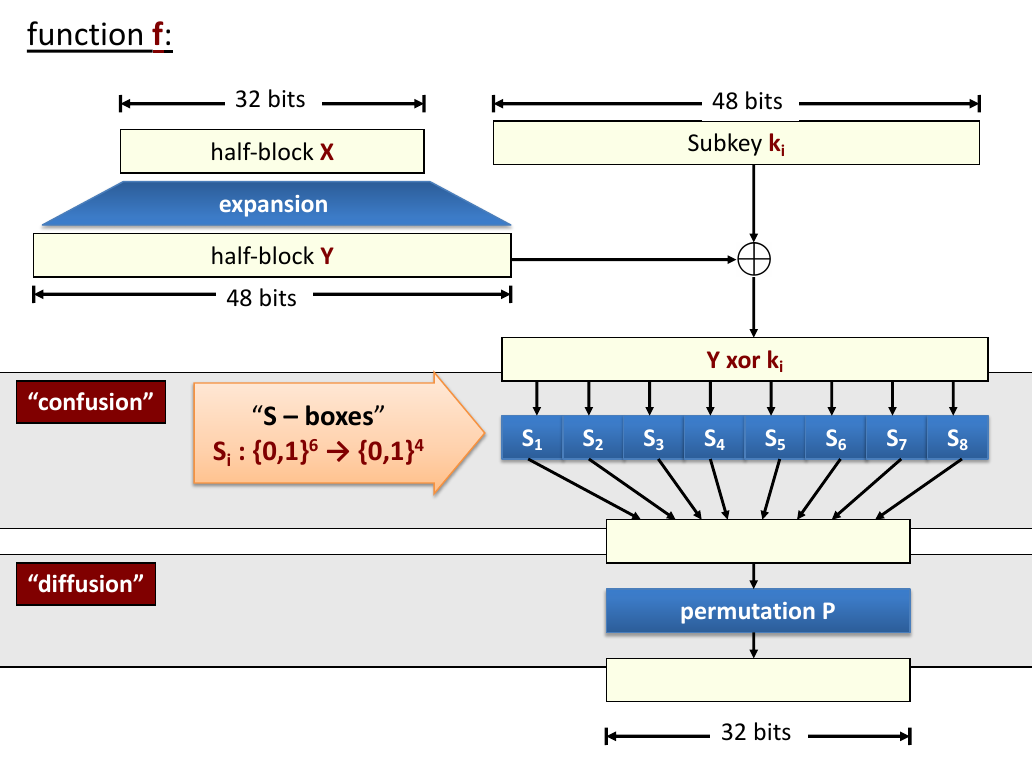
\includegraphics[width=8cm]{images/ch2-expansion-substitution-permutation.png}
    \caption{Expansion, substitution and permutation}
    \label{fig:exp-subst-perm}
\end{figure}

\paragraph{Feistel network}
see Figure \ref{fig:feistel-network}. To decrypt, reverse the key schedule.
% https://www.overleaf.com/learn/latex/Inserting_Images
\begin{figure}[h]
    \centering
    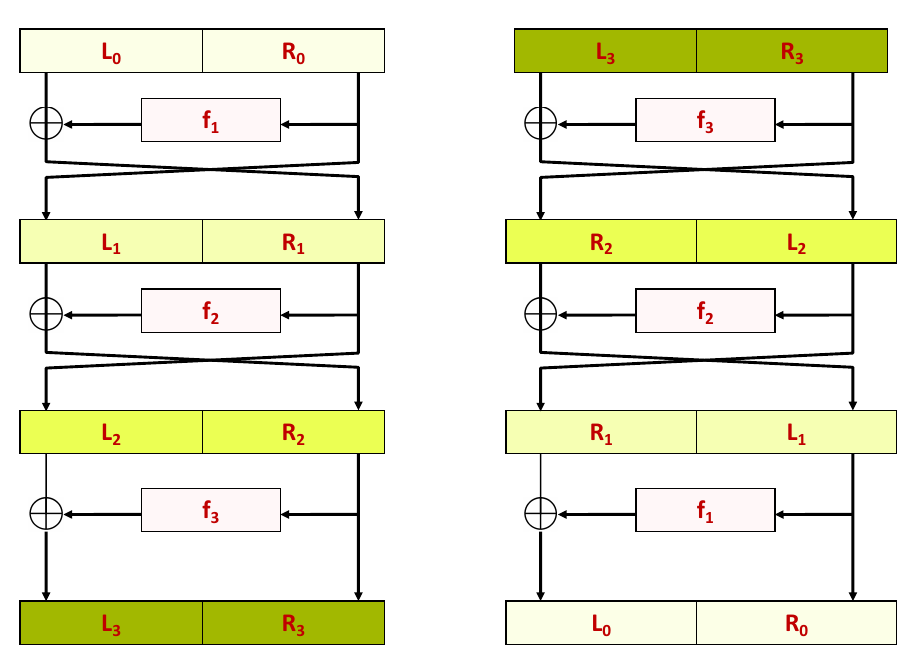
\includegraphics[width=8cm]{images/ch2-feistel-network.png}
    \caption{Feistel network. LHS encryption, RHS decryption.}
    \label{fig:feistel-network}
\end{figure}

\paragraph{Increasing key size} Double encryption ($F'_{(k, k')}(x) = F_{k'}(F_{k}(x))$) can easily be attacked with \textit{Meet-in-the-middle} attack (given PT/CT pairs, try all possible keys to encrypt half way and all keys to decrypt from the other side, find matching pairs in the list to find valid key).

Instead triple encryption ($F'_{(k_1, k_2, k_3)}(x) = F_{k_3}(F^{-1}_{k_2}(F_{k_1}(x)))$) is preferred. It is NOT immune to the meet-in-the-middle attack but it takes significantly longer. 

\paragraph{Product cipher} Cascading (repeatedly applying) a cipher, e.g. to increase key size.


\subsection{Block cipher modes of operation}

\paragraph{Electronic Codebook (ECB)} Every block is encrypted identically $\implies$ same plaintext results in same ciphertext, thus \textbf{NOT SECURE}.

\paragraph{Cipher-Block Chaining (CBC)} Use initialization vector (IV) to XOR the first plaintext block before applying the actual encryption function, the resulting cipher is used to XOR the plaintext of the next block, and so on. Need to use different IV for every message. The IV and the propagation through the blocks makes sure that the same data does not result in the same cipher.

\textbf{Theorem}: If $F$ is a PRP then $F$-CBC is secure.\footnote{thgoebel: The slides do not mention which secureness? I assume IND-CPA secure?}
\\ \\
The follow two modes aim at converting a pseudorandom permutation (PRP) into a pseudorandom generator (PRG) $G$:

\paragraph{Output Feedback (OFB)} Use seed and PRF to generate one-time-pad (OTP) to use for first block, use the OTP of the first block to generate the OTP for the second block, and so on. The OTPs are then XORed with the respective message block. Generally not parallelisable, but the OTPs can be precomputed. IND-CPA secure if $F$ is a PRP.

$G(k, IV) = F_k(IV) || F_k(F_k(IV)) || F_k(F_k(F_k(IV))) || ... $\footnote{The notation $||$ means "concatenation".}

\paragraph{Counter (CTR)} Use $IV+i$ and PRF to generate OTP for respective message block (i.e. OTP for block $i$ is given by $F_k(IV + i)$). IND-CPA secure.

$G(k, IV) = F_k(IV+1) || F_k(IV+2) || F_k(IV+3) || ... $

\begin{table}[h]
    \centering
    % https://tex.stackexchange.com/questions/39435/how-can-i-center-a-too-wide-table/39436#39436
    \addtolength{\leftskip} {-2cm}
    \addtolength{\rightskip}{-2cm}
    \begin{tabular}{|l||c|c|c|c|}
    \hline
    & ECB & CBC & OFB & CTR \\ \hline \hline
    Error propagation: transmission\\ error in block $c_i$ affects... & only block $c_i$ & only $c_i$ and $c_{i+1}$ & only block $c_i$ & only block $c_i$ \\ \hline
    Encryption parallelisable & $\checkmark$ & $\times$ & $\times$ & $\checkmark$ \\ \hline
    Decryption parallelisable & $\checkmark$ & $\checkmark$ & $\times$ & $\checkmark$ \\ \hline
    If 1 bit in plaintext changes,\\ recompute ... & 1 block\tablefootnote{Leaks information!} & everything & 1 block & 1 block \\ \hline
    \end{tabular}
    \caption{Comparison of block cipher modes of operation}
    \label{table:block-modes}
\end{table}

\begin{figure}[h!]
    \centering
    \addtolength{\leftskip} {-5cm}
    \addtolength{\rightskip}{-5cm}
    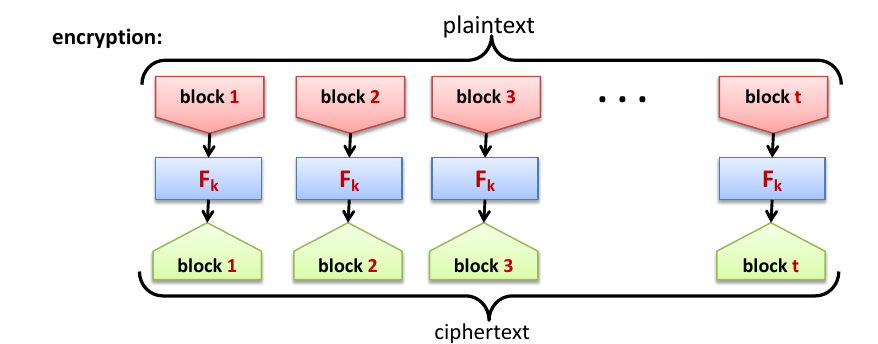
\includegraphics[width=9cm]{images/ch2-bc-ecb-enc.png}
    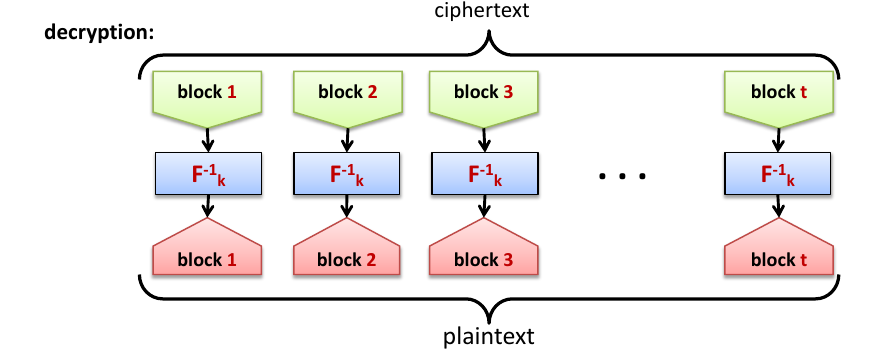
\includegraphics[width=9cm]{images/ch2-bc-ecb-dec.png}
    \caption{Electronic Codebook ECB}
    \label{fig:bc-ecb}
\end{figure}
\begin{figure}[h!]
    \centering
    \addtolength{\leftskip} {-5cm}
    \addtolength{\rightskip}{-5cm}
    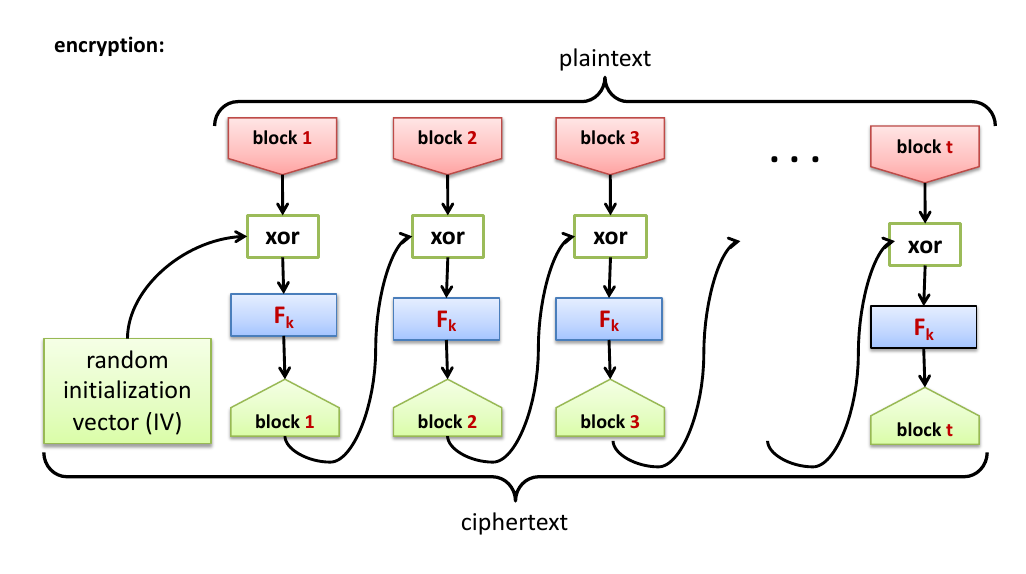
\includegraphics[width=9cm]{images/ch2-bc-cbc-enc.png}
    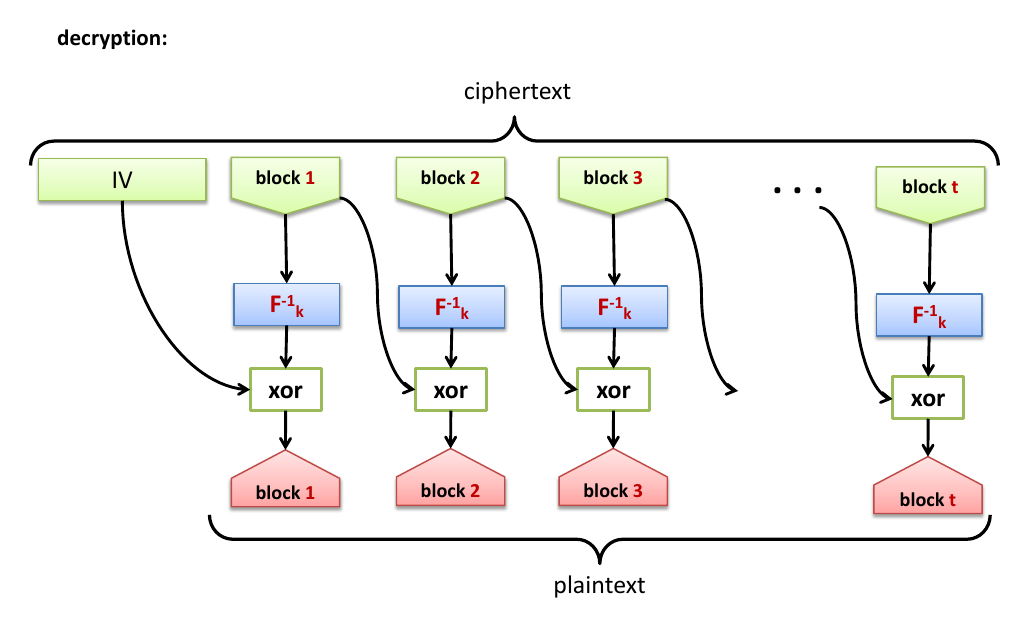
\includegraphics[width=9cm]{images/ch2-bc-cbc-dec.png}
    \caption{Cipher-Block Chaining CBC}
    \label{fig:bc-cbc-enc}
\end{figure}
\begin{figure}[h!]
    \centering
    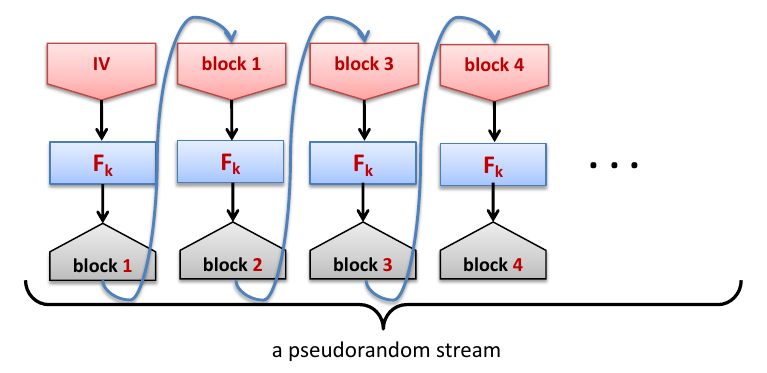
\includegraphics[width=9cm]{images/ch2-bc-ofb.png}
    \caption{Output Feedback OFB}
    \label{fig:bc-ofb}
\end{figure}
\begin{figure}[h!]
    \centering
    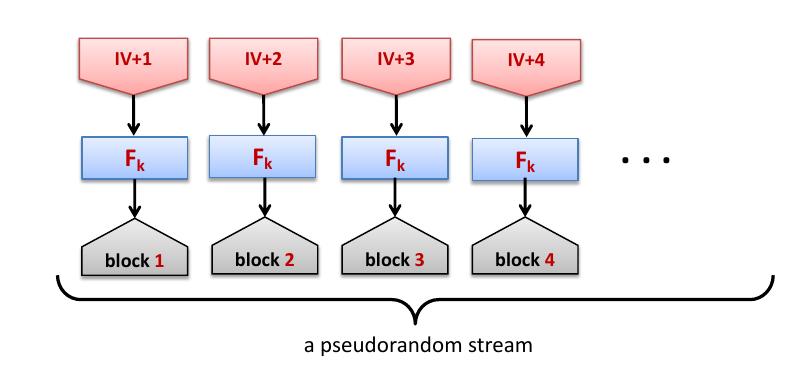
\includegraphics[width=9cm]{images/ch2-bc-ctr.png}
    \caption{Counter CTR}
    \label{fig:bc-ctr}
\end{figure}

\paragraph{Self-recovering} A mode where errors don't propagate, e.g. CBC

\paragraph{Padding} If the length of the message is not evenly divisible by the block size, we need to expand the message to fit the block size. This is achieved through adding some data to the end of the message or through \textit{ciphertext stealing}.

\paragraph{Initialisation vector (IV)} Random input to a block cipher. Sent to the recipient together with the ciphertext. Enables key reuse.

\paragraph{Seed} Input to a PRG. Sometimes this term is used instead of "IV", not always a clear distinction.
\\ \\
Summary graph: \\
PRP/PRF exists $\xRightarrow[]{\text{modes of operation}}$ secure encryption exists $\Rightarrow$ one-way functions exist $\Rightarrow$ wraparound: PRP/PRF exists\footnote{TODO: Can somebody draw a nice diagram?}


%
% CHAPTER 3
%
\newpage
\section{Stream Ciphers}

\subsection{Pseudorandom Generators}

\paragraph{Pseudorandom Generator PRG} $G: \setzeroone^* \mapsto \setzeroone^* $ such that
$$\forall n \forall s \text{ with } |s|=n : \; |G(s)| = l(n)$$
where $l$ is a polynomial with $\forall n: \; l(n) > n$ and for a random $s$ then $G(s)$ "looks random" too. $s$ is called the \textbf{seed} and $l$ the \textbf{expansion factor}.

\begin{figure}[h]
    \centering
    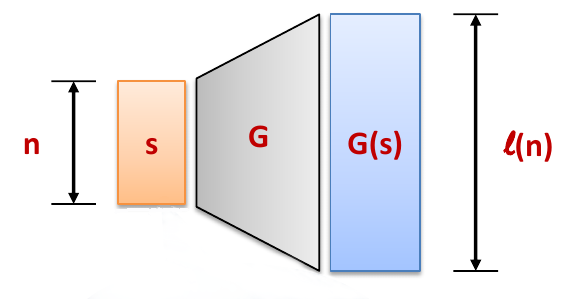
\includegraphics[width=6cm]{images/ch3-sc-prg.png}
    \caption{Pseudorandom Generator PRG}
    \label{fig:sc-prg}
\end{figure}

Notice that if $s$ is chosen uniform at random (from $\setzeroone^n$) then $G(s) \in \setzeroone^{l(n)}$ cannot be u.a.r.

\paragraph{Cryptographic PRG} PRG such that every PPTTM can only distinguish $G(S)$ from a $R$ with $p=0.5 + \varepsilon$; where $S$ is distributed u.a.r. over $\setzeroone^n$ and $R$ is distributed u.a.r. over $\setzeroone^{l(n)}$ and $\varepsilon$ is negligible.

\paragraph{Golomb's Postulate}
\begin{enumerate}
    \item $|$Number of 1s -- number of 0s in $G(s)| \leq 1$
    \item "Run" of 0s (or 1s) of length $i$ occurs with $p=2^{-i}$
    \item some maths ...
\end{enumerate}

\paragraph{Theorem} Cryptographic PRG exists $\implies$ computationally-secure encryption exists (proof by a tight reduction).

\paragraph{One-way function} A function $f:\; \setzeroone^* \mapsto \setzeroone^*$ is one-way if it is 1) poly-time computable and 2) invertible by a poly-time adversary with negligible probability.

\paragraph{Theorem} $P=NP \implies$ one-way functions do NOT exist.\footnote{The proof is left as an exercise.}\\
However there are some candidates, like prime factorisation: $f(p,q)=p\cdot q$.

\paragraph{Remark} One-way functions do NOT hide all the input! The following is a valid one-way function:
$$ f(x_0,...,x_{n-1}, x_n) = f'(x_0, ... , x_{n-1}) || x_n $$

\begin{figure}[h!]
    \paragraph{Theorem} One of the most fundamental results in symmetric cryptography: \\
    \begin{center}
        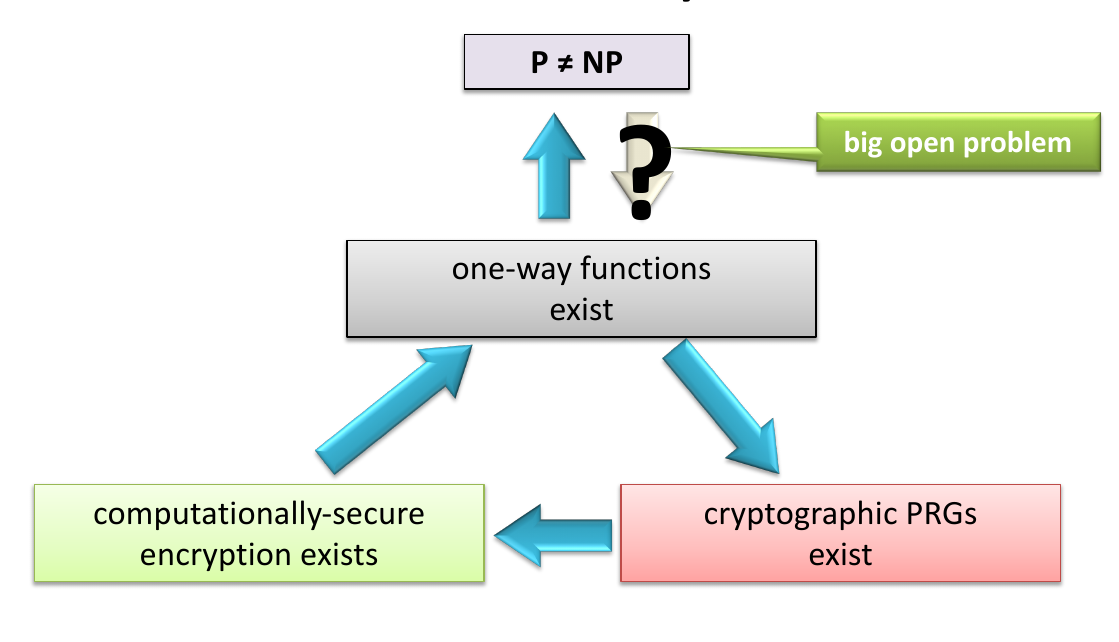
\includegraphics[width=9cm]{images/ch3-sc-one-way.png}
        \caption{Relation between one-way functions, cryptographic PRGs and computationally-secure encryption}
        \label{fig:sc-one-way}
    \end{center}
\end{figure}



\subsection{Stream ciphers in practice}

\paragraph{Stream ciphers} output "infinite" streams of bits (as opposed to a number of blocks).

The challenge in using PRGs for encryption is that we cannot reuse the same seed - see the one-time pad! So instead:

\paragraph{Synchronised mode} Divide $G(s)$ into blocks and xor them with blocks of plaintexts. CPA-secure. Difficult in practise because it requires keeping state (where in $G(s)$ were we?).

\paragraph{Unsynchronised mode} Randomise by using a PRG $G(IV_i, s)$ that takes an additional input $IV_i$ (fresh for each message $m_i$).

For this we can either design such a $G$ from scratch or use a cryptographic hash function $H$ (see chapter \ref{section-hash-fucntions}): $G(IV, s) \coloneqq G'(H( IV||s )) $.

\begin{figure}[h]
    \centering
    \addtolength{\leftskip} {-5cm}
    \addtolength{\rightskip}{-5cm}
    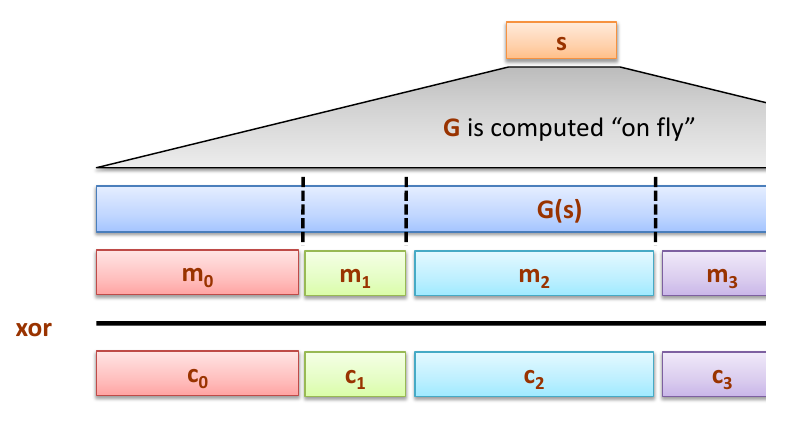
\includegraphics[width=7cm]{images/ch3-sc-sync.png}
    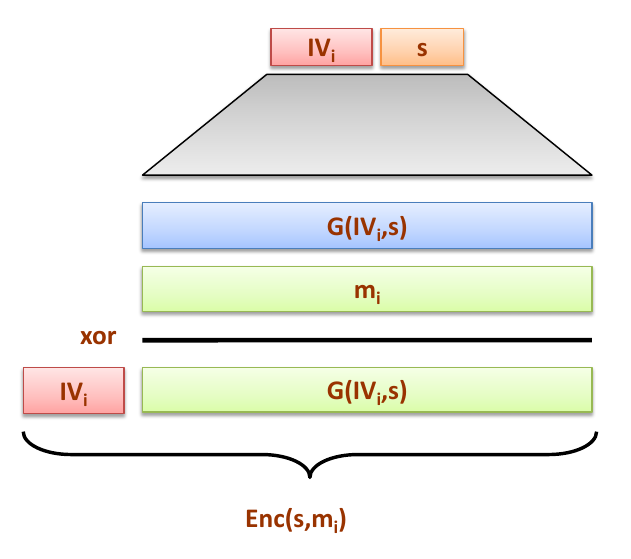
\includegraphics[width=7cm]{images/ch3-sc-unsync.png}
    \caption{Synchronised (left) and unsynchronised mode (right)}
    \label{fig:sc-sync-unsync}
\end{figure}

\paragraph{RC4} Old but once widely used stream cipher. No security intuition, no proof! Problems:
\begin{enumerate}
    \item No $IV$ per default. Implementation specific: a) WEP uses an $IV$ but too short (repeats after a day). b) Others reset $IV$ on each restart...
    \item Some output bytes are biased.
    \item First bytes of output can leak information about the key.
    \item Too short key lengths in some implementations (e.g. WEP) $\implies$ brute-forceable
\end{enumerate}

\paragraph{ChaCha, Salsa} Modern stream ciphers. Fast in software (as opposed to HW-accelerated AES). Addition/Rotation/XOR (ARX) make linear and differential cryptanalysis difficult. Combination in step 3 (see figure \ref{fig:sc-chacha}) gives hard-to-inverseability.

\begin{figure}[h]
    \centering
    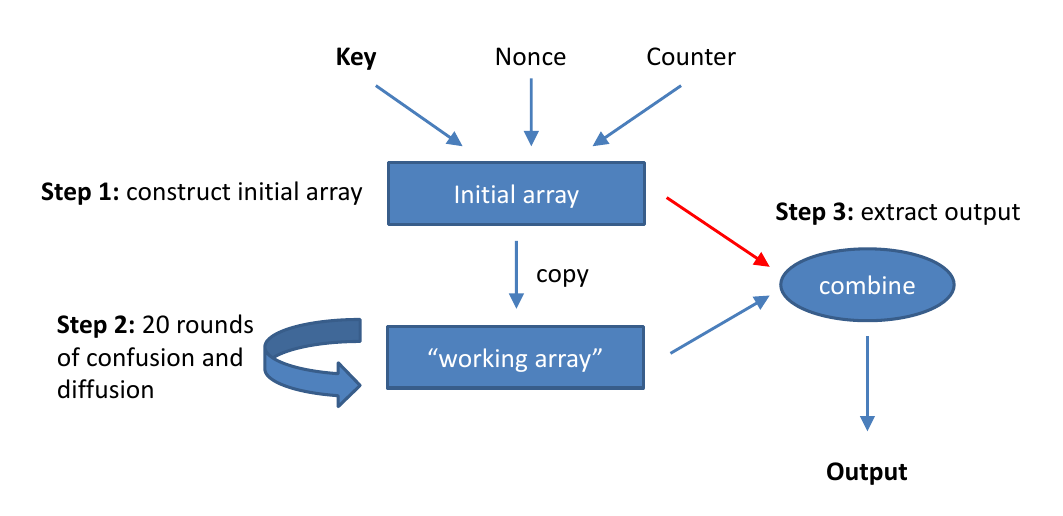
\includegraphics[width=9cm]{images/ch3-sc-chacha.png}
    \caption{ChaCha schematics}
    \label{fig:sc-chacha}
\end{figure}



%
% CHAPTER 4
%
\newpage
\section{Hash Functions and MACs}

\subsection{Message Authentication}

\paragraph{Integrity}
How can Bob be sure that $m$ really comes from Alice and has not been tampered with?

\paragraph{Message Authentication Code (MAC) scheme} is a pair $(\operatorname{Tag}, \operatorname{Vrfy})$ where 

$\operatorname{Tag}:  \mathcal{K} \times \mathcal{M} \rightarrow \mathcal{T}$ is a tagging algorithm

$\operatorname{Vrfy}:  \mathcal{K} \times \mathcal{M} \times \mathcal{T} \rightarrow \{\textit{yes}, \textit{no}\}$ is a verification algorithm.

\underline{Correctness:} $\operatorname{Vrfy}_k(m,\operatorname{Tag}_k(m)) = \textit{yes}$ should always hold.

\paragraph{Remark} MACs per se do not protect against \textbf{replay attacks}. A simple workaround would be to include a timestamp in the message.

\paragraph{MAC security} A given MAC is secure, if 
$$\forall \text{ probabilistic poly-time adversaries } \mathcal{A}: \; P [ \mathcal{A} \text{ breaks } MAC ] = \varepsilon(n) $$
i.e. breaks it with probability negligible in the key size $n$. \textit{Breaks} mean $\mathcal{A}$ produces a valid $(m', t')$ pair for an unseen message $m'$.

\paragraph{Construction of a secure MAC} using block ciphers:

For one block: $\operatorname{Tag}_k(m) = F_k(m)$ (provable secure)

Generalising to multiple blocks: 

\begin{enumerate}
    \item Prepend counter to every block (to avoid permutation by adversary)
    \item Include message length in every block (to avoid truncation)
    \item Add a (per message) fresh random value to each block (to avoid splicing of different same-length messages)
\end{enumerate}

Using all these measures results in a provable secure MAC. However, this construction is not practical. One Problem is that the tag is 4 times longer than the message, we need 4 times as many invocations of $F_k$.

\paragraph{CBC-MAC} see figure \ref{fig:cbc-mac}

If we would not prepend $|m|$ then the adversary could forge $ (m', t') = (m_1 || m_2 \oplus t_1, t_2) $ (after learning $(m_1, t_1)$ and $(m_2, t_2)$ in a training phase). This is known as a \textit{splicing attack}.

\begin{figure}[h]
    \centering
    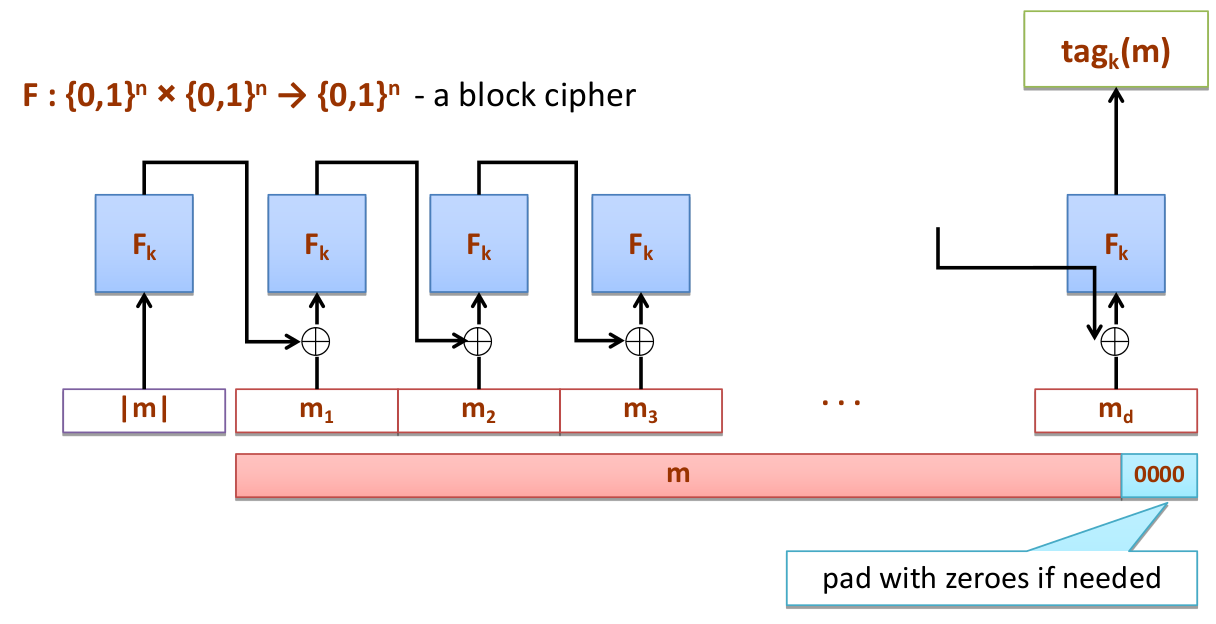
\includegraphics[width=10cm]{images/ch4-cbc-mac.png}
    \caption{CBC-MAC}
    \label{fig:cbc-mac}
\end{figure}

\paragraph{Disadvantages of block-cipher-based MAC} compared to hash functions-based MACs:

\begin{itemize}
    \item Less efficient
    \item Many protected by export regulations
\end{itemize}



\subsection{Hash functions} \label{section-hash-fucntions}

The basic property required for a hash function is collision resistance. Collisions always exist since the domain is much larger than the range the function maps to.

\paragraph{Collision resistance} It should be "hard" to find a pair $(m, m')$ such that $H(m) = H(m')$.

\paragraph{Security definition} $H$ is a collision-resistant hash function, if 
$$\forall \text{ poly-time adversary }\mathcal{A}: \Pr[\mathcal{A} \text{ breaks } H] = \varepsilon(n)$$
The oracle selects $s$ u.a.r., $A$ outputs $(m, m')$. We say that adversary $A$ breaks $H$, if $H^s(m) = H^s(m')$.

\underline{Problem:} for fixed $H$ there always exists an algorithm that finds a collision in constant time, because the hashing algorithm is fully known. Workaround: we use a key $s$.

\paragraph{Hash function} A hash function is a probabilistic polynomial-time algorithm $H$ such that:

$H$ takes as input a key $s \in \{0, 1\}^n$ and a message $x \in \setzeroone^*$ and outputs a string $H^s(x) \in \{0,1\}^{L(n)}$ where $L(n)$ is some fixed function.\footnote{In reality, a hash function only takes a message as an input. The key only denotes the concrete instantiation out of the \textit{family} of hash functions $H^s$.}

\paragraph{Hash-based MAC} A key for MAC is a pair $(s, k)$. $s$ is a key for hash function $H$ and $k$ for PRP $F$. 
$$\operatorname{Tag}((s, k), m) = F_k(H^s(m))$$
\textit{Theorem:} If $H$ and $F$ are secure, then $\operatorname{Tag}$ is secure (proof by reduction).

\paragraph{Constructing hash functions} 

\begin{enumerate}
    \item Construct a smaller fixed-input-length collision-resistant hash function $h$ (aka. the \textit{compression function}). 
        $$h: \{0, 1\}^{2L} \rightarrow \{0,1\}^L$$
    \item Use $h$ to construct a variable length hash function $H$.
        $$H: \{0, 1\}^{*} \rightarrow \{0,1\}^L$$
\end{enumerate}

\paragraph{Constructing a compression function} Common approaches:

\begin{itemize}
    \item block cipher
    \item specially designed function, e.g. SHA
    \item use Feistel Network as basis
\end{itemize}

\paragraph{Merkle-Damgard transform} see figure \ref{fig:damgard-merkle}. Note that $|m| = t$, $|m_i| = |IV| = |L|$. We append $m_{B+1} \coloneqq t$ to prevent padding attacks.

\textit{Theorem:} If $h$ is a collision-resistant compression function, then $H$ is a collision-resistant hash function.

\begin{figure}[h]
    \centering
    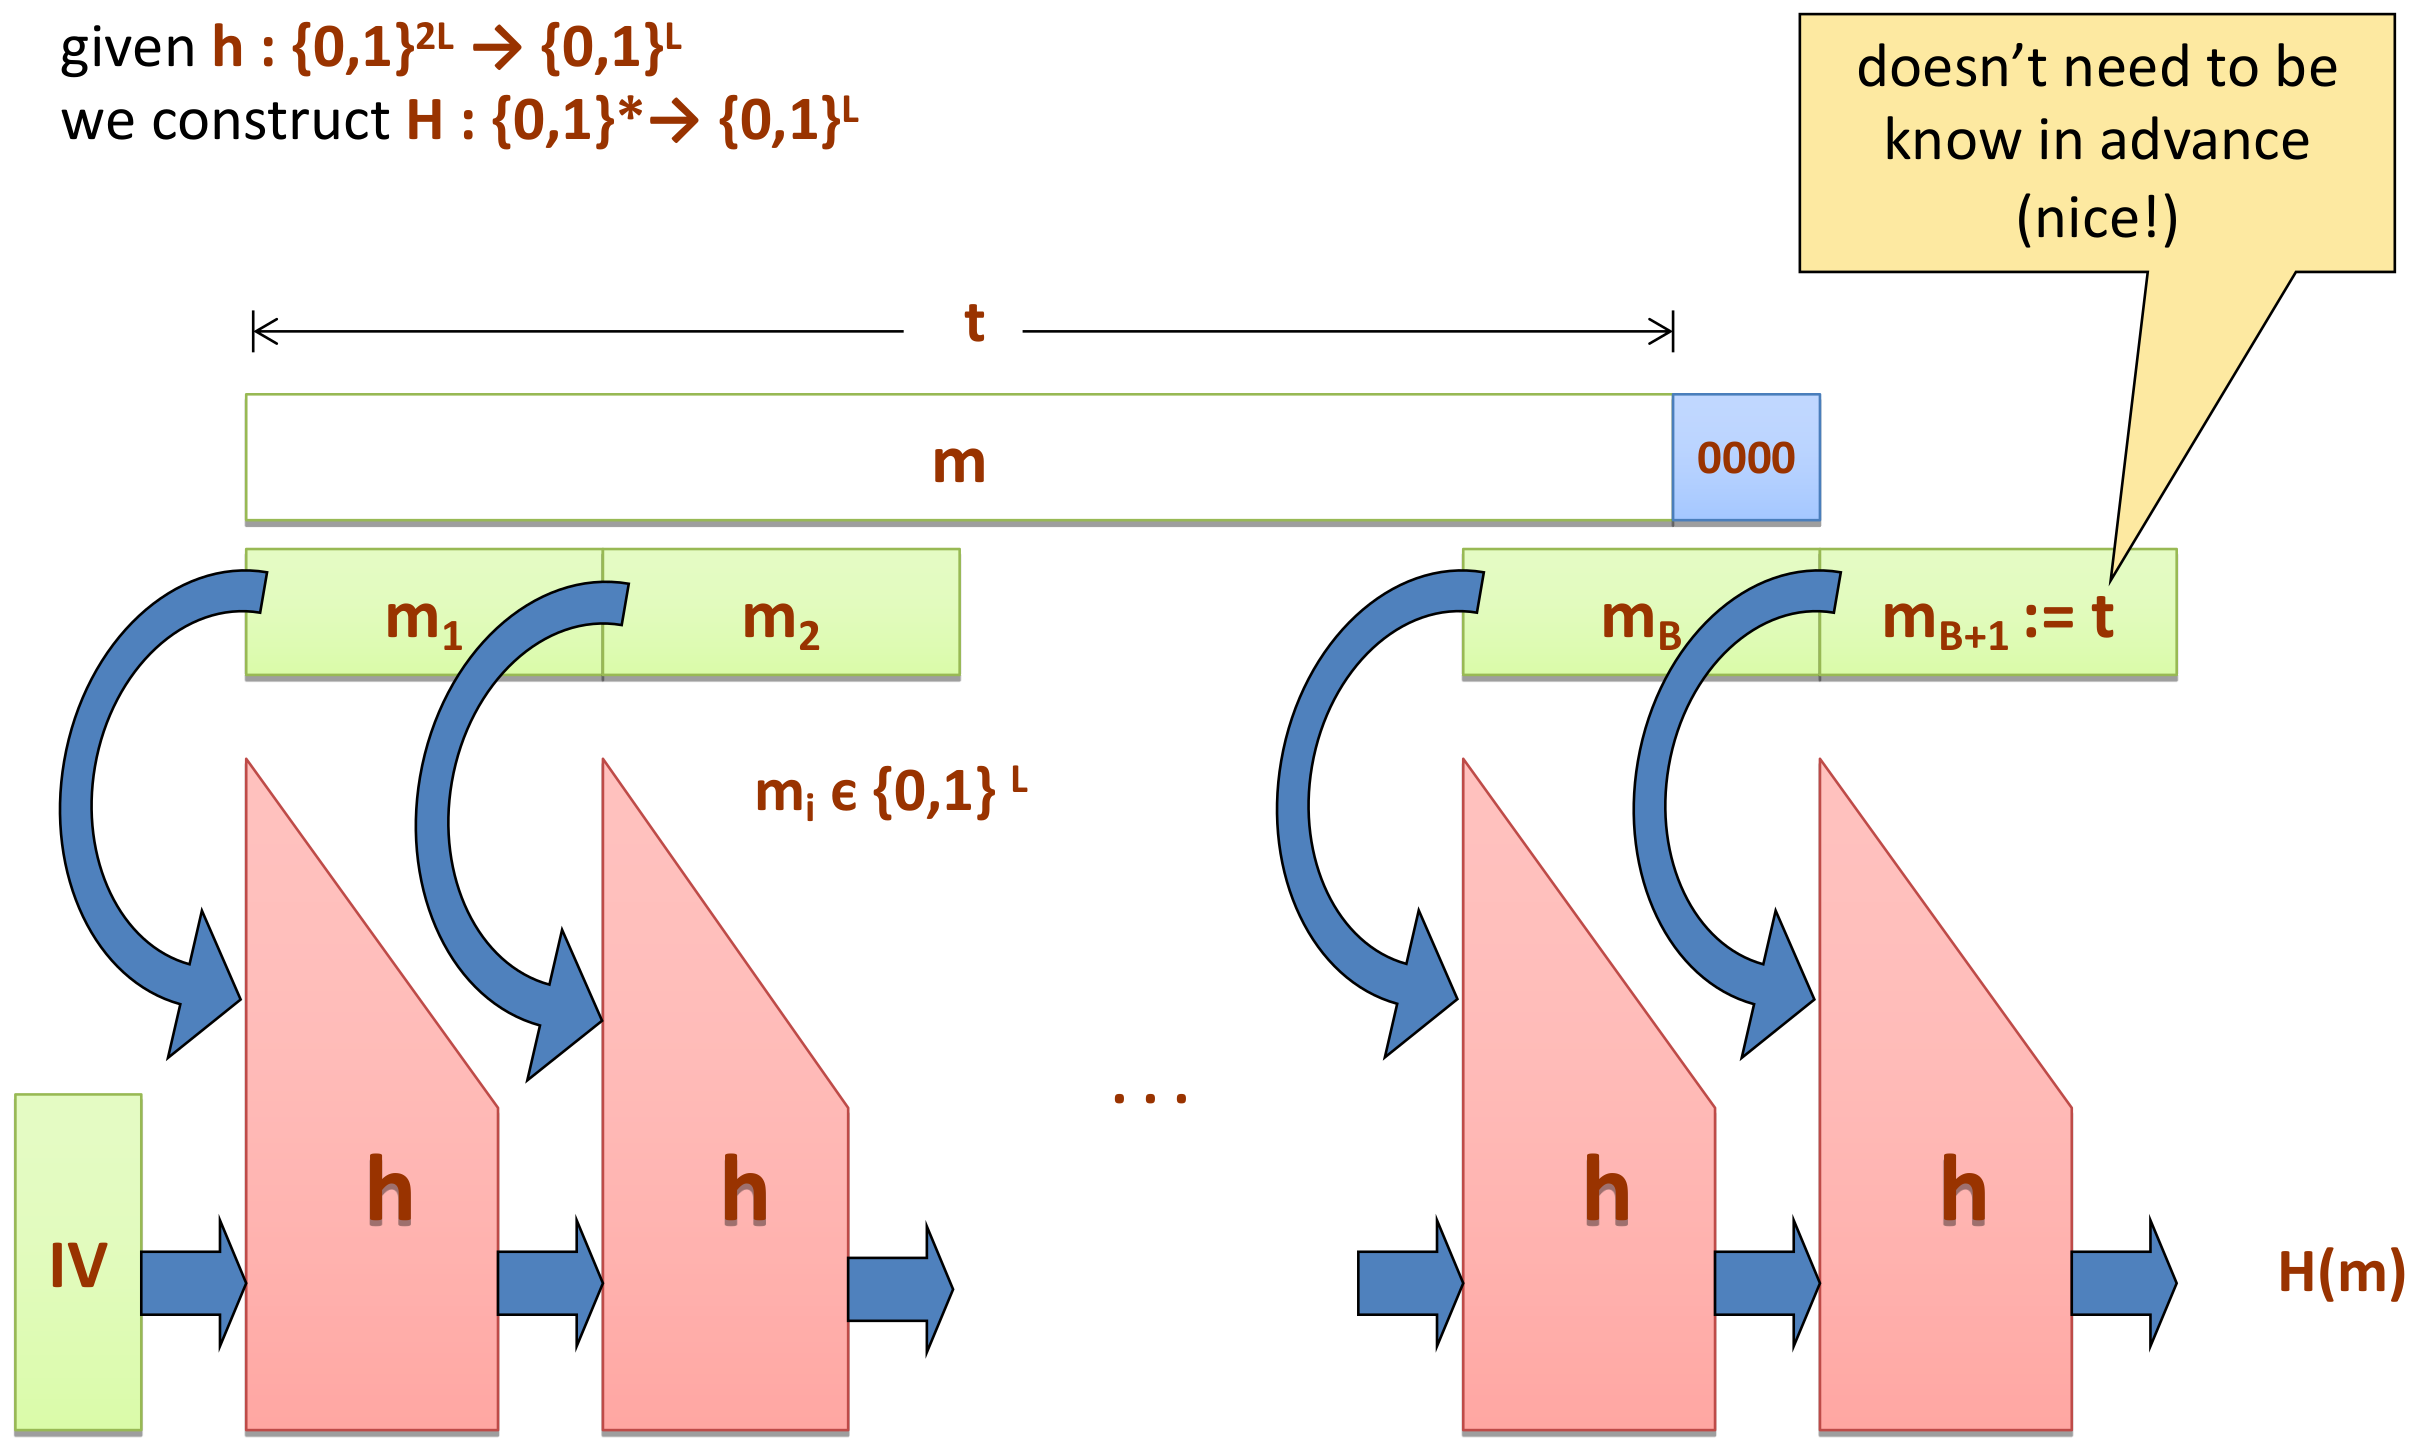
\includegraphics[width=10cm]{images/ch4-damgard-merkle.png}
    \caption{Merkle-Damgard construction}
    \label{fig:damgard-merkle}
\end{figure}

\paragraph{Concrete hash functions} MD5 (broken), SHA-1 (broken), SHA-256, SHA-3 (does not use Merkle-Damgard, uses 'sponge construction') 

\paragraph{Other Hash Function Properties} Weaker security notions than collision
resistance:

\begin{itemize}
    \item \underline{Preimage resistance:} Given hash value $v$, find $x$ such that $h(x) = v$ ("inverting")
    \item \underline{$2^{\text{nd}}$ preimage resistance:} Given $x$, find $x' \neq x$ such that $h(x) = h(x')$
\end{itemize}

Collision Resistance $\Rightarrow$ Preimage resistance

Collision Resistance $\Rightarrow$ $2^{\text{nd}}$ preimage resistance

\paragraph{Nested MAC (NMAC)} see figure \ref{fig:nmac}. Takes two keys $k_1, k_2$.

\underline{Disadvantages of NMAC}

\begin{itemize}
    \item Most real-world hash functions (MD5, SHA-1) do not permit to change IV (they use a fixed IV)
    \item The key $(k_1, k_2)$ is too long
\end{itemize}

\begin{figure}[h]
    \centering
    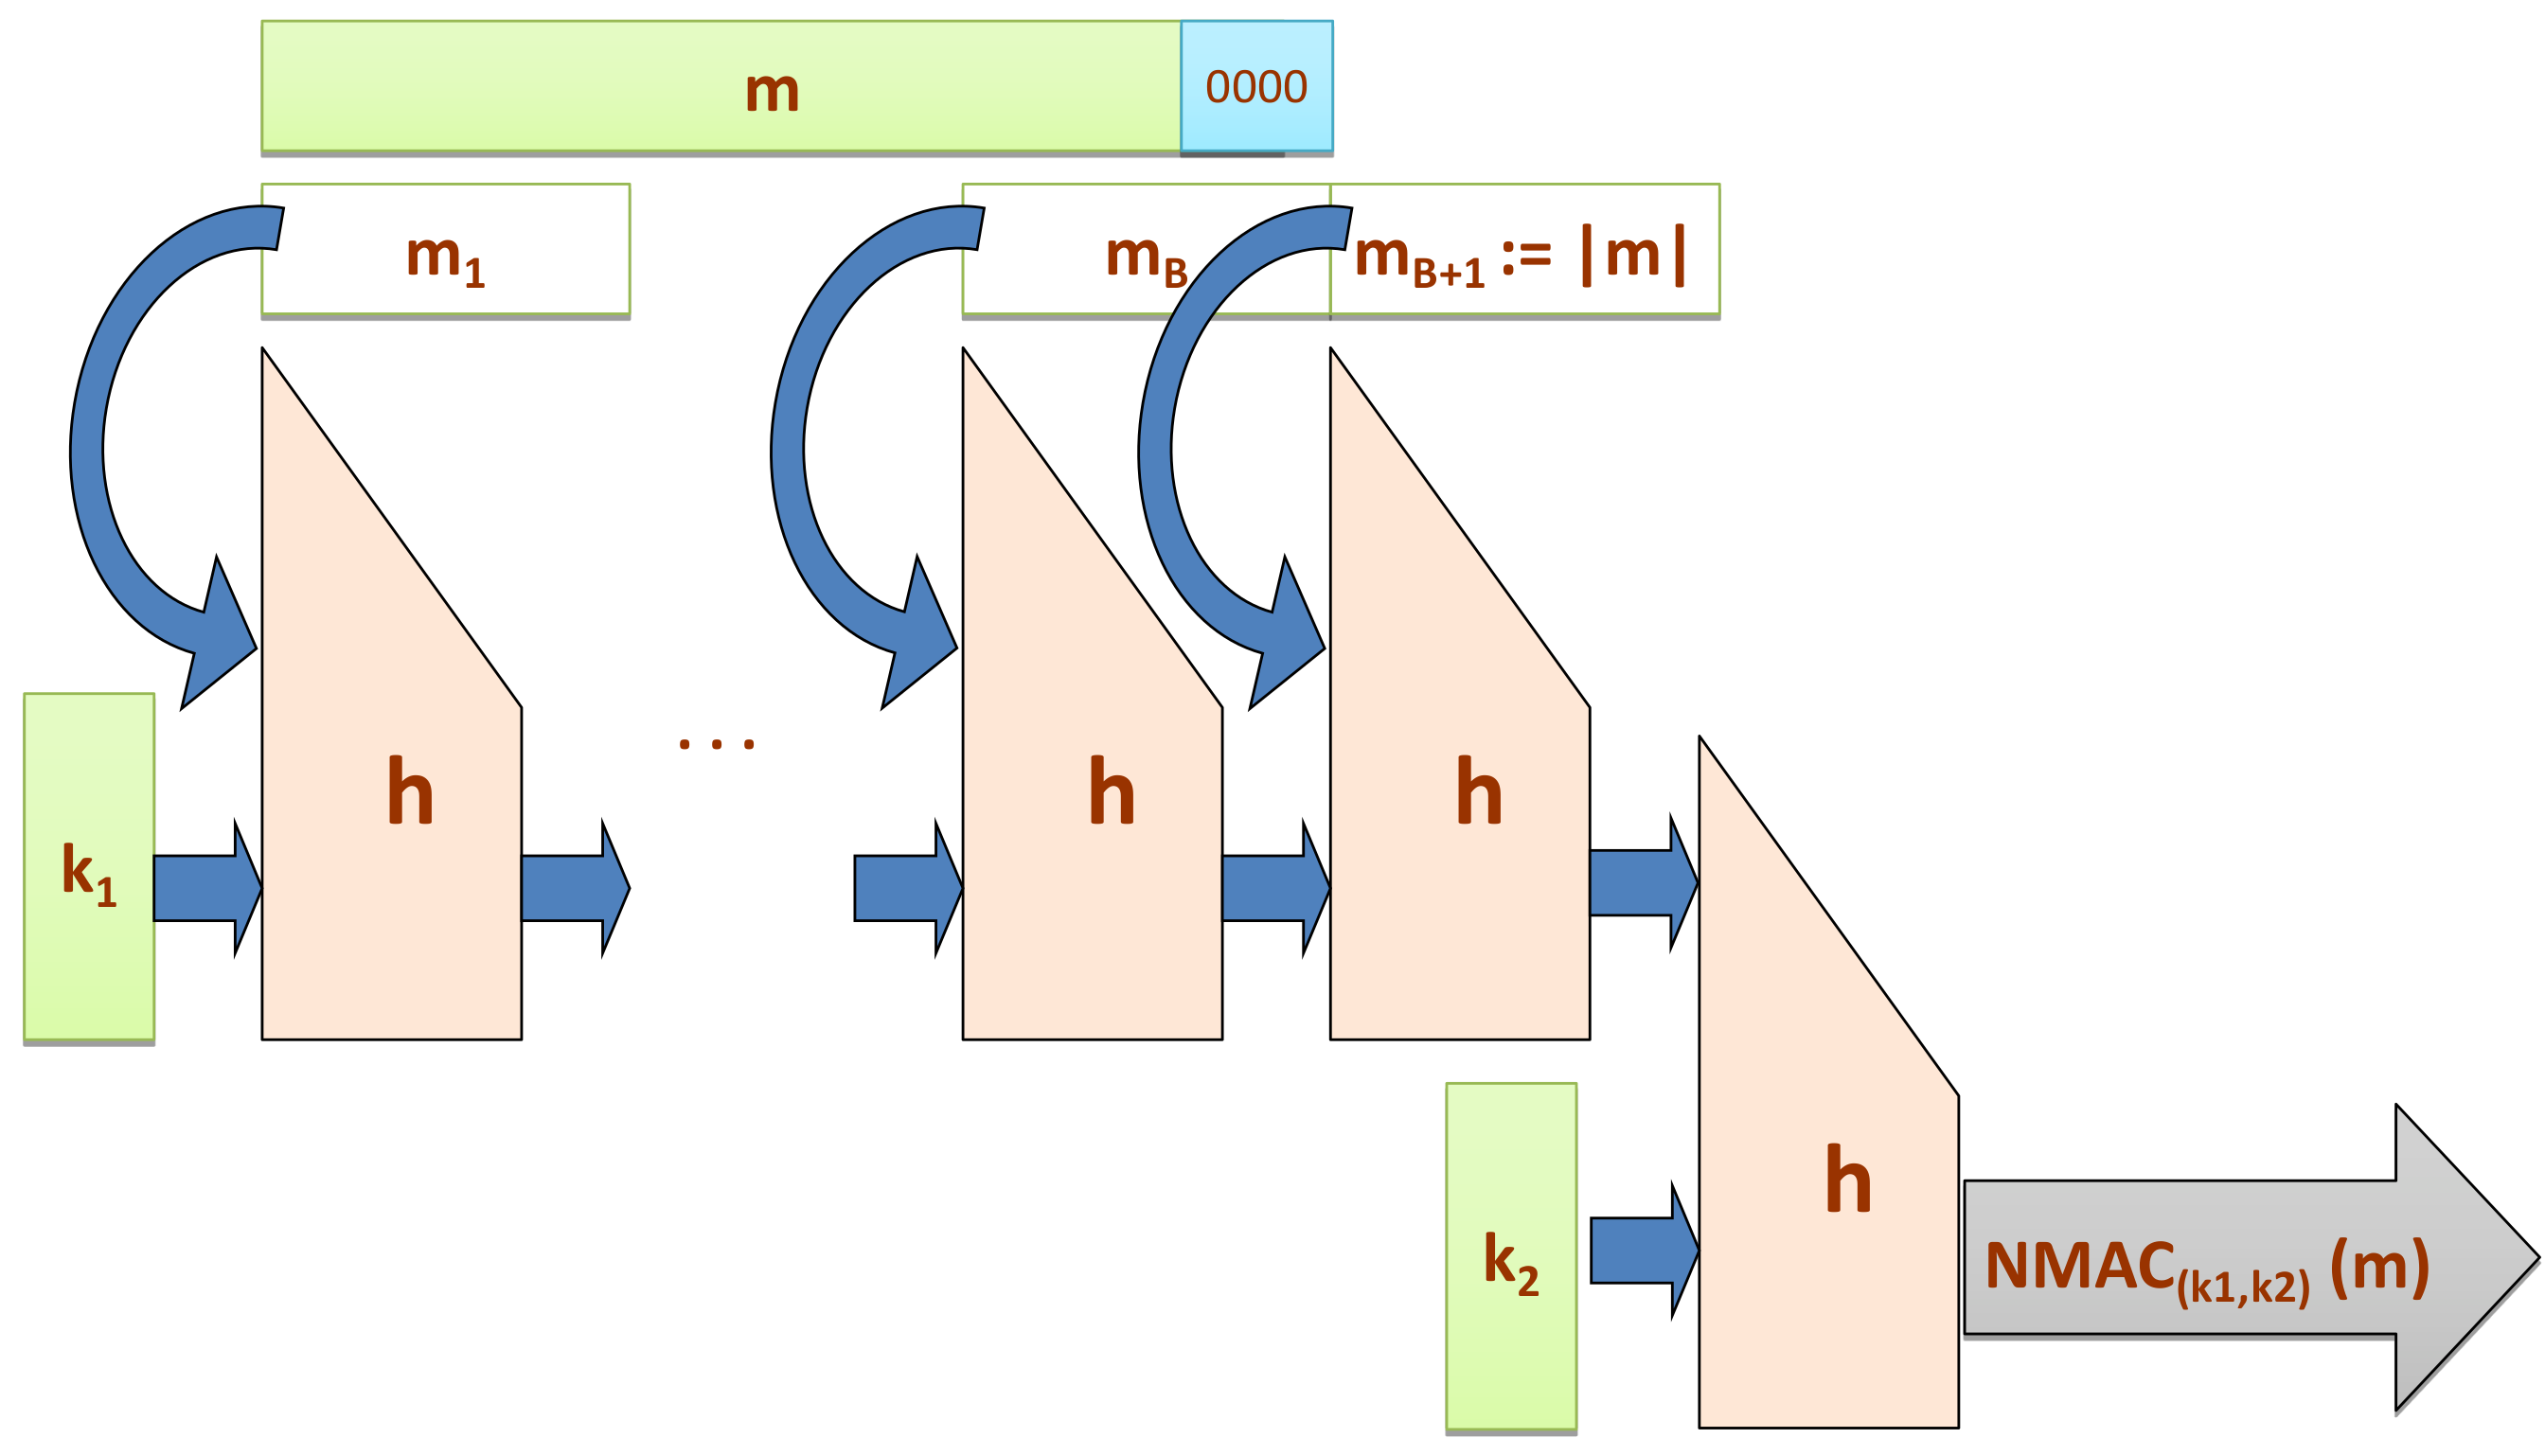
\includegraphics[width=10cm]{images/ch4-nmac.png}
    \caption{NMAC}
    \label{fig:nmac}
\end{figure}

\paragraph{Hash-based MAC (HMAC)} see figure \ref{fig:hmac}

\underline{Advantages of HMAC}

\begin{itemize}
    \item Easy to implement given $H$:
        $$ \operatorname{HMAC}_k(m) = H\big( (k \oplus \text{opad} ) \; || \; H(k \oplus \text{ipad}\; || \; m ) \big) $$
        \item Has provable properties
        \item Is widely used in practice
\end{itemize}

\begin{figure}[h]
    \centering
    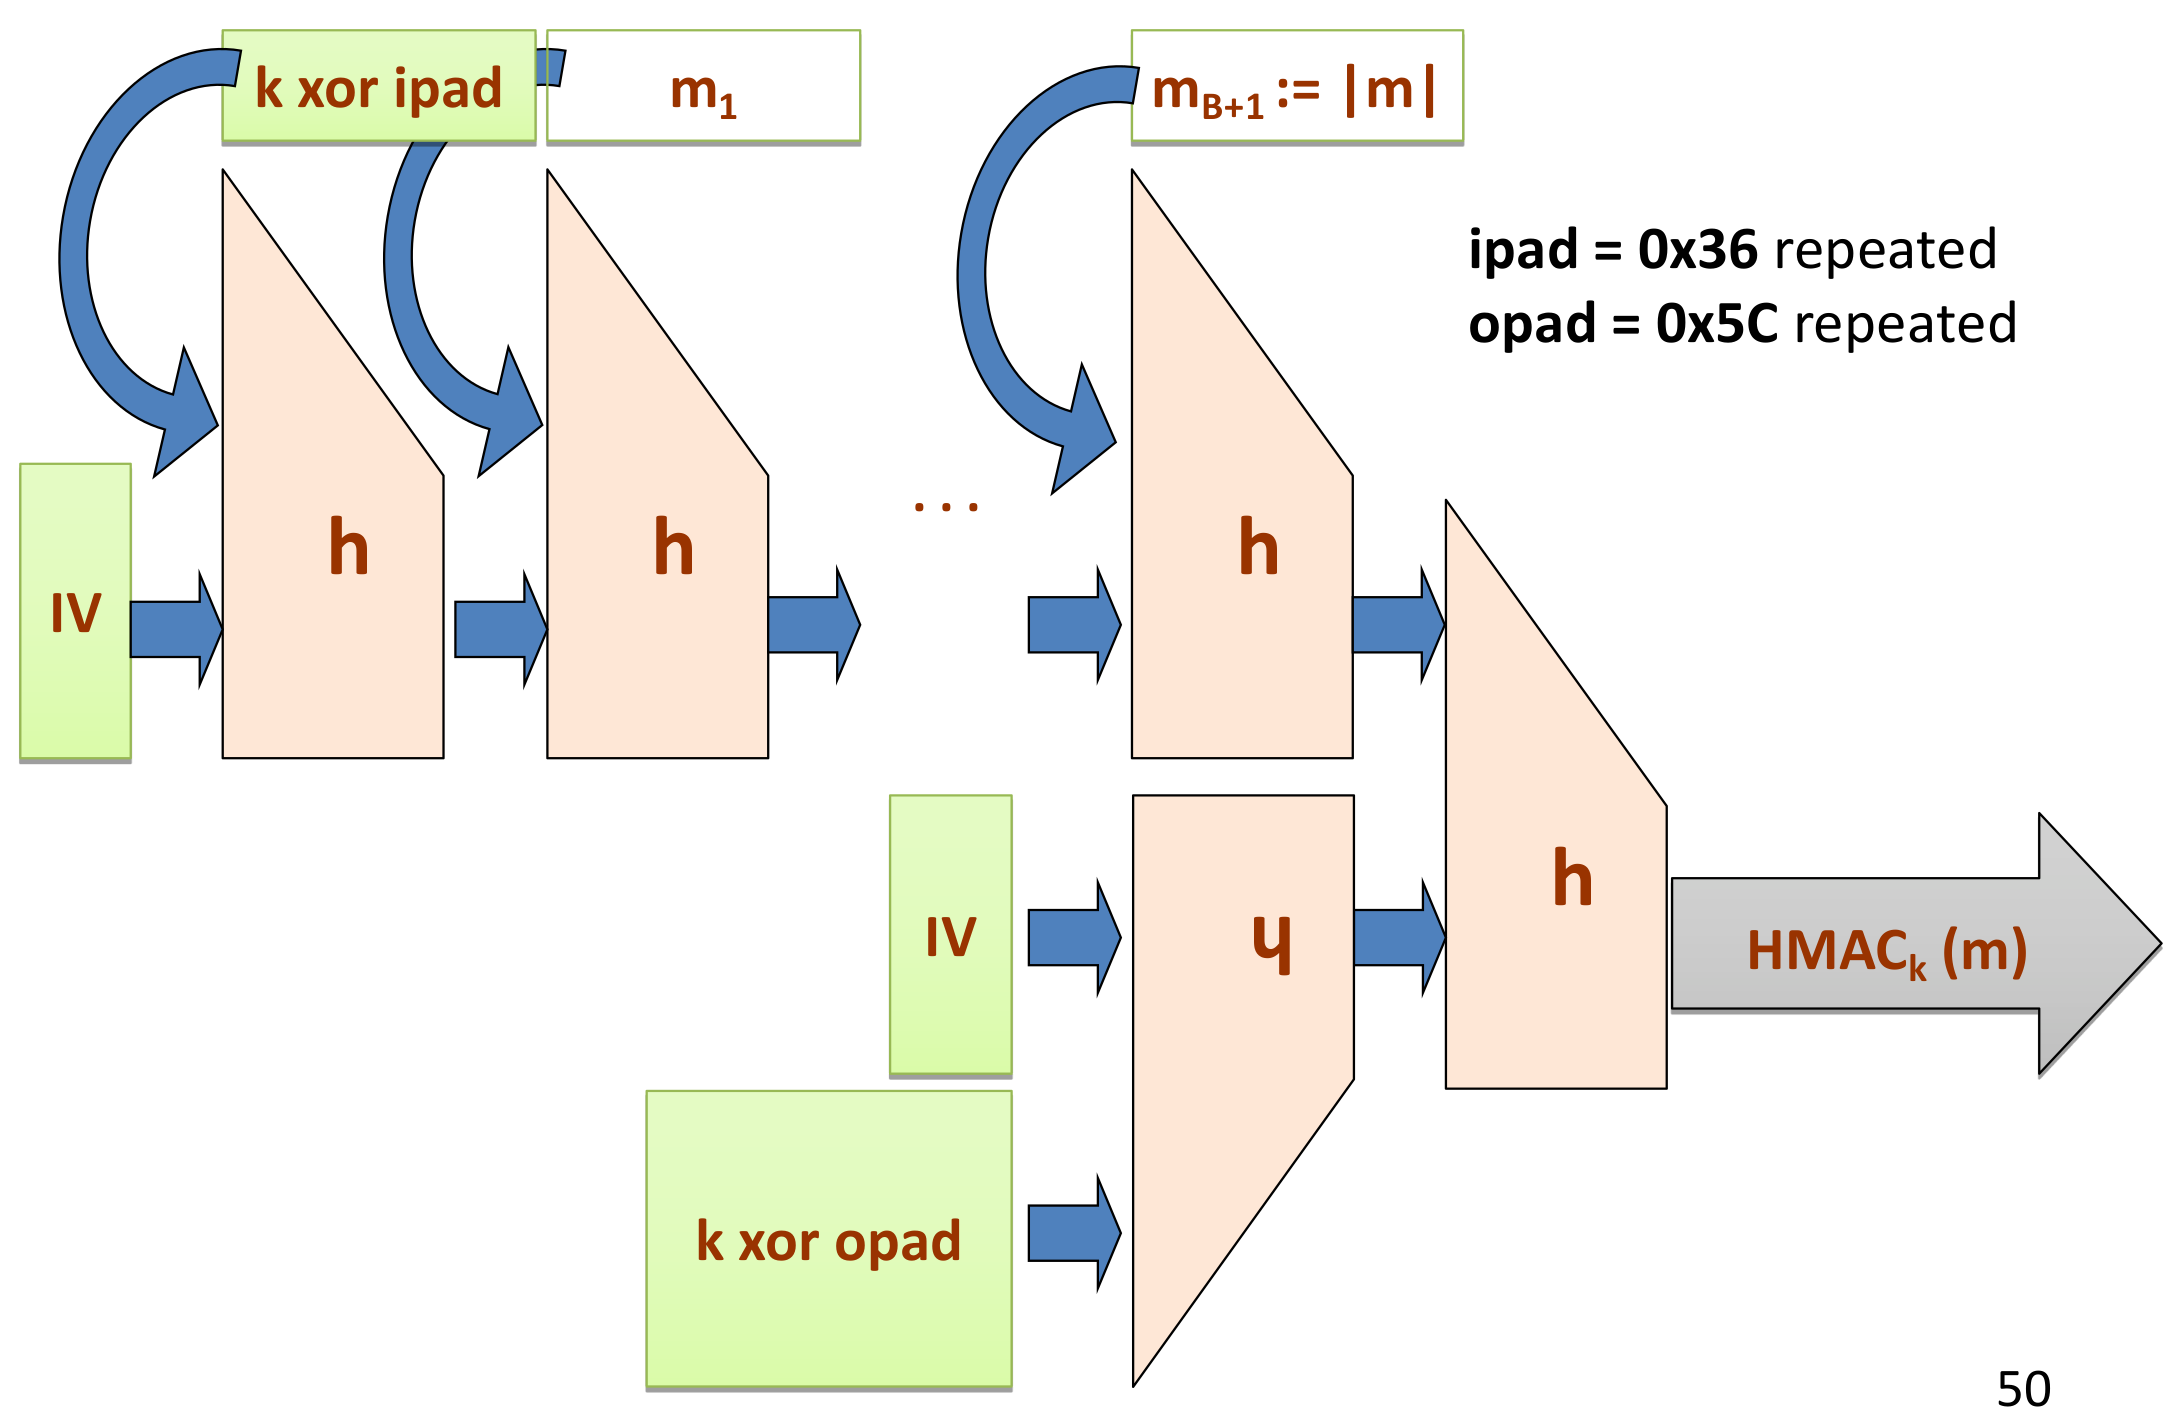
\includegraphics[width=10cm]{images/ch4-hmac.png}
    \caption{HMAC}
    \label{fig:hmac}
\end{figure}

\paragraph{Other uses} Hash functions are used in practice to convert “non-uniform randomness” into a uniform one.



%
% CHAPTER 5
%
\newpage
\section{Public-Key Cryptography}

\paragraph{The idea} Instead of using one key $k$, we use two keys $(pk, sk)$, where $pk$ (public) is used for encryption and $sk$ (private) is used for decryption.

\underline{Advantages of public keys}: Simplified key management, i.e.

\begin{itemize}
    \item secrecy not required
    \item fewer keys (Alice can use the same pair to communicate with multiple parties)
\end{itemize}

\paragraph{PKC for authentication} $sk$ is used for computing a tag (\textit{signature}) and $pk$ is used for verifying correctness of the tag. 

\underline{Advantages of signature schemes:}

\begin{itemize}
    \item publicly verifiable\footnote{With symmetric MACs, Carol cannot verify that $(m, \operatorname{Tag}_k(m))$ comes from Alice and is only relayed by Bob. She cannot verify that $(m, \operatorname{Tag}_k(m))$ was not indeed created by Bob (given $k$ is shared between Alice and Bob).}
    \item transferable
    \item provides non-repudiation (one cannot deny having signed $m$)
\end{itemize}

\paragraph{Trapdoor permutations} A trapdoor permutation is a family of permutations indexed by $pk \in \mathcal{K}$;
$$ \{\operatorname{Enc}_{pk}: \mathcal{M} \rightarrow \mathcal{C}\}_{pk \in \mathcal{K}} $$
such that for every key $pk$, there exists a key $sk$, and it is:
\begin{itemize}
    \item easy to compute $\operatorname{Enc}_{pk}$
    \item easy to compute $\operatorname{Enc}_{pk}^{-1} = \operatorname{Dec}_{sk}$ if one knows a trapdoor $sk$
    \item hard to compute $\operatorname{Enc}_{pk}^{-1} = \operatorname{Dec}_{sk}$ otherwise
\end{itemize}

\paragraph{PKC in practise: number theory} We make use of mathematical problems that are known to be hard (hardness assumption). A suitable area of math is number theory.

\underline{Advantages of using number theory}

\begin{itemize}
    \item Security can (in principle) be based on famous mathematical conjectures.
    \item Constructions have a “mathematical structure”. This allows us to create more advanced constructions (public key encryption, digital signature schemes, etc ...).
    \item Constructions have a natural security parameter: \textbf{size} (hence they can be “scaled”).
    \item (A wonderful argument for theoreticians: a practical application of an area that was never believed to be practical.)
\end{itemize}

\underline{Disadvantages of using number theory}

\begin{itemize}
    \item Cryptography based on number theory is much less efficient.
    \item The number-theoretic “structure” can help the cryptanalysis.
    \item Certain problems that are believed to be hard for classical computers are shown to be easy for quantum computers.
\end{itemize}

\paragraph{Cyclic groups} (Easy way there) Let $G$ be a group, $g \in G$, $i$ be the order of $g$.

Then the cyclic group $\langle g \rangle ~= \{g^0, g^1,\dots,g^{i-1}\}$ is a subgroup of $G$ generated by $g$.

Notabene:
\begin{itemize}
    \item Closed under multiplication: $g^a \cdot g^b = g^{a+b \operatorname{mod} i}$
    \item Inverse always exist\footnote{Proof left as an exercise.}: $(g^a)^{-1} = g ^{i-a}$
    \item $g^x$ can easily be computed using \textit{square-and-multiply}
\end{itemize}

\paragraph{Discrete logarithms} (Hard way back) Suppose $G$ is cyclic, and $g$ is its generator. For every element $y$, there exists $x$ such that 
$$y = g^x$$
Such a $x$ will be called a \textit{discrete logarithm} of $y$, and is denoted as $x \coloneqq \log y$.

\paragraph{Hardness assumption of the discrete logarithm}
In some groups\footnote{Groups of numbers, not groups of mathematicians!}, computing a discrete logarithm is believed to be hard. This includes:

\begin{itemize}
    \item $Z_p^* = \{ 1, ..., p-1 \}$ where $p$ is prime
    \item groups based on elliptic curves
\end{itemize}

\textit{Note:} $P = NP$ implies computing the discrete logarithm is easy.

\underline{Formal definition}

Let $H$ be an algorithm. Given input $1^n$, $H$ outputs a description of a group $G$ of order $q$, such that $q = n$.
% Note that it is NOT $|q| = n$, this was an error on the slides!

Oracle: Let $(G, g)$ be the output of $H(1^n)$. The oracle selects a random element $y \leftarrow G$ from the group and returns $(G, g, y)$ to the adversary.

A discrete logarithm problem is hard with respect to $H$, if
$$\forall \text{ probabilistic poly-time adversary } \mathcal{A}: \Pr[\mathcal{A} \text{ outputs } x \text{ s.t. } y = g^x)] = \varepsilon(n)$$


\subsection{Diffie-Hellman key exchange}\label{section-dh-exchange}

\paragraph{Key exchange} Protocol through which two parties that initially share nothing can establish a shared secret despite the presence of an intermediate adversary.

\paragraph{Diffie-Hellman key exchange} Let $G$ be a group where discrete log is believed to be hard, let $q = |G|$, and let $g$ be a generator of $G$. See figure \ref{fig:dh} for the key exchange protocol.

\begin{figure}[h]
    \centering
    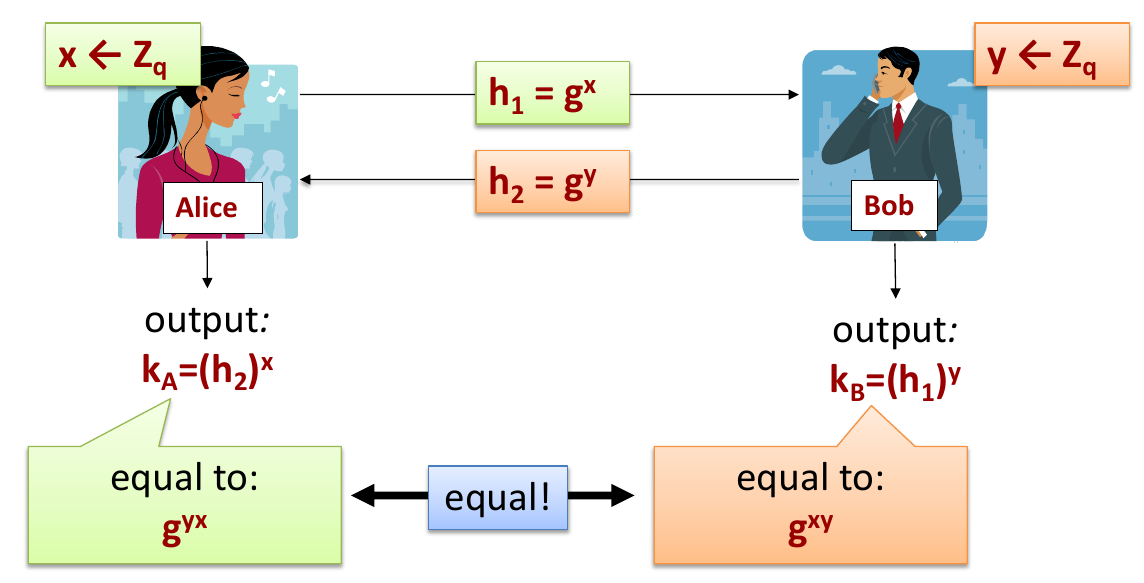
\includegraphics[width=11cm]{images/ch5-dh.png}
    \caption{Diffie-Hellman key exchange}
    \label{fig:dh}
\end{figure}

\paragraph{Security of a key exchange protocol}\mbox{}

\textit{Informally:} (Alice, Bob) is secure if no adversary can distinguish $k$ from a random sequence $r$, given the transcript $T$ of sent messages, with a non-negligible advantage.

\textit{Formally:} We say $(\text{Alice}, \text{Bob})$ is a secure key exchange protocol if: the output (key) of Alice and Bob is always the same, and 
$$\forall \text{ probabilistic poly-time adversary } \mathcal{A}: |\Pr[\mathcal{A}(1^n,k) = 1] - \Pr[\mathcal{A}(1^n,r) = 1]| = \varepsilon(n)$$

Is DH secure?

\begin{enumerate}[label=\Alph*)]
    \item If the discrete log in $G$ is easy, then the DH key exchange is \underline{not} secure.
    \item If the discrete log in $G$ is hard, then it may also be insecure.
\end{enumerate}

\paragraph{Quadratic residue QR} $y \in G$ is a \textit{quadratic residue} if there exists an $a \in G$ such that $a^2 = y$.

\Lightning \mbox{} Testing whether $y \in Z_p^*$ is a QR is possible in polynomial time. \\
$\implies$ An adversary observing $y = g^x$ can learn whether $x$ is even (iff $y$ is QR) or odd, i.e. information about the parity of $k$ is leaked: $k = g^{xy}$ is QR iff any of $g^x$ and $g^y$ is QR. \\
$\implies$ Diffie-Hellman key exchange is \underline{not} secure  in $Z_p^*$!

\paragraph{Decisional Diffie-Hellman assumption}
$$\forall \text{ PPT adversary } \mathcal{A}: |\Pr[\mathcal{A}(G, g, q, g^x, g^y, g^{xy}) = 1] - \Pr[\mathcal{A}(G, g, q, g^x, g^y, g^r) = 1]| = \varepsilon(n)$$
where $r$ is random.

This does \underline{not} hold in $Z^*_p$ but it is believed to be hard in $QR_p$ (which is a subgroup of $Z^*_p$ such that $p$ is a safe prime).

\paragraph{Safe prime} $p$ is a \textit{safe prime} if $p = 2q + 1$, where $q$ is also prime.

\paragraph{Man-in-the-middle attack} Adversary that is not passively eavesdropping on the messages but is actively intercepting and manipulating them. Diffie-Hellman is \underline{not} secure against it.


\subsection{ElGamal encryption scheme}

\paragraph{ElGamal encryption} Encryption scheme which for each message runs a Diffie-Hellman key exchange to generate a new shared key. This key is then used to encrypt a single message. See figure \ref{fig:elgamal}.

\paragraph{Security of ElGamal} If DDH is hard relative to $G$, then ElGamal is CPA-secure (under a \underline{passive} adversary!).

\begin{figure}[h]
    \centering
    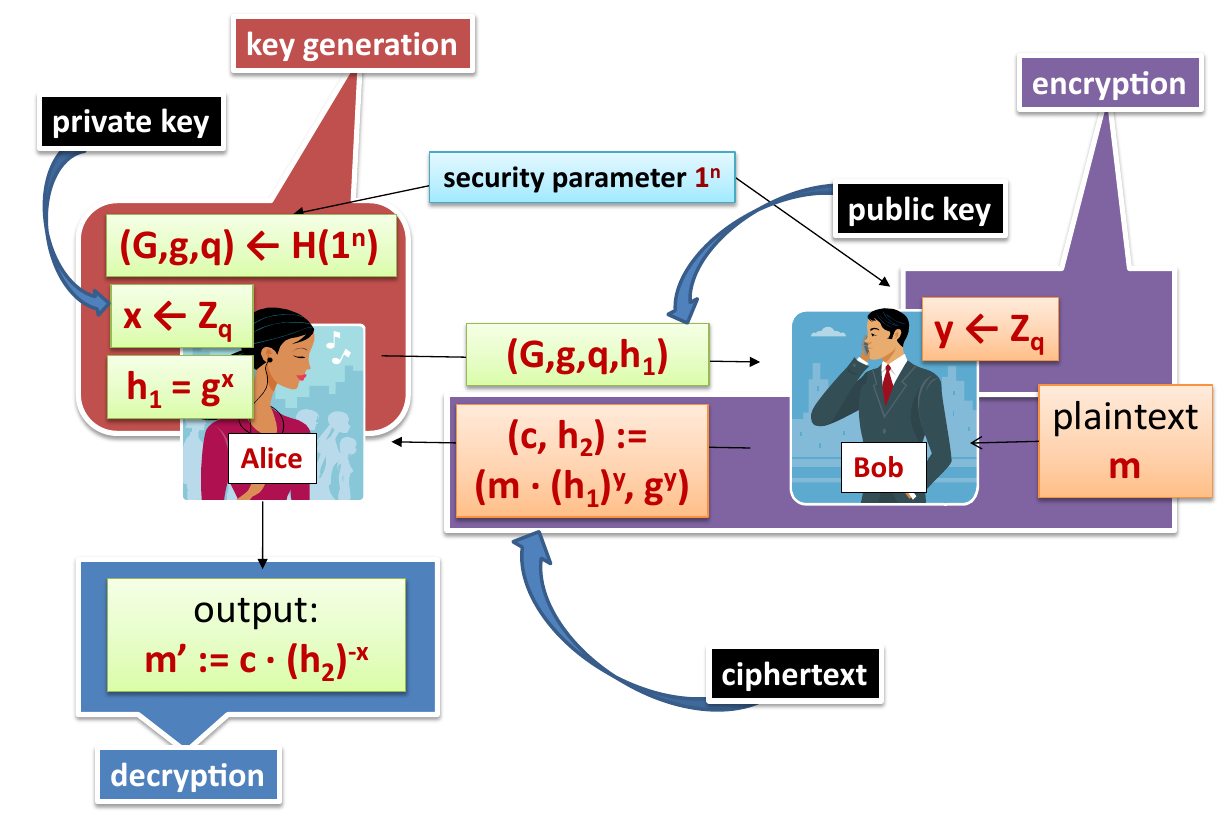
\includegraphics[width=11cm]{images/ch5-elgamal.png}
    \caption{ElGamal encryption scheme}
    \label{fig:elgamal}
\end{figure}


\subsection{RSA encryption scheme}

\paragraph{RSA key generation} Given a security parameter $1^n$:

\begin{enumerate}
    \item Choose two prime numbers $p$ and $q$ of size $n$
    \item Compute $N = pq$
    \item Compute totient\footnote{Euler's totient function $\Phi(N)$ gives the number of integers smaller than $N$ that are relatively prime to $N$. Recall that two numbers $a, b$ are relatively prime if $\operatorname{gcd}(a,b) = 1$.} $\Phi(N) = (p-1)(q-1)$
    \item Choose $e$ relative prime to $\Phi(N)$, i.e. $\gcd(e, \Phi(N))=1$
    \item Compute $d = e^{-1} \mod \Phi(N)$ (i.e. $d$ is multiplicative inverse of $e$, modulo $\Phi(N)$)
\end{enumerate}

This yields a public key $pk = (e, N)$ and a private key $sk = (d, N)$. Note that $p$, $q$ and $\Phi(N)$ remain secret.

\paragraph{RSA encryption \& decryption} \mbox{}

encryption: $$c \coloneqq m^e \mod N$$ 
decryption: $$m \coloneqq c^d \mod N$$

\paragraph{RSA encryption security} Intuition: If attacker could factor $N$ to $p$ and $q$ then she could:
\begin{itemize}
    \item first compute $\Phi(N) = (p-1)(q-1)$ and
    \item then find the private key $d = e^{-1} \mod \Phi(N)$
\end{itemize}

$\Rightarrow$ Computing $\Phi(N)$ cannot be more difficult than factoring

Claim: computing $\Phi(N)$ is as hard as factoring N.

Proof outline: Suppose we can compute $\Phi(N)$. Then we know that $ (p-1)(q-1) = \Phi(N)$ and $pq = N$. This is a system of 2 equations with 2 unknowns. It can easily be solved analytically for $p$ and $p$.

\paragraph{RSA assumption} It is hard to compute the $e$\textsuperscript{th} root (of $c$) without knowing $\Phi(N)$. 

Or formally: 
$$\forall \text{ PPT algorithm } \mathcal{A}:  \Pr\big[m^e = c \mod N \; | \; m = \mathcal{A}(c, N, e)\big] = \varepsilon(|N|) = \varepsilon(k)$$

where $N = pq$ with $p$ and $q$ random primes and $|p| = |q| = k$, $c$ is a random element of $Z_N^*$, and $e$ is random element of $Z_{\Phi(N)}^*$ with $\gcd(e, \Phi(N))=1$.

\paragraph{CPA security in a public-key cryptosystem}
The is no need for a training phase with the oracle -- knowing $pk$, the adversary can do the training herself.

\paragraph{Issues with "textbook" RSA}
\begin{itemize}
    \item \textbf{NOT CPA-secure:} No deterministic public key encryption scheme is! The adversary can simply do the encryption of the messages $m_0, m_1$ (which she gives to the oracle) herself and compare $c_0$ and $c_1$ to the $c$ she got back from the oracle. Thus she can output $b$ correctly with $p=1$.
    \item \textbf{Homomorphic:} $$ RSA_{e,N}(m_0\cdot m_1) = (m_0\cdot m_1)^e = m_0^e \cdot m_1^e = RSA_{e,N}(m_0) \cdot RSA_{e,N}(m_1) $$
    Using this the adversary can find out whether the to-her-unknown $m, m_0, m_1$ are related through $m_0 \cdot m_1 = m$ by checking whether $c_0 \cdot c_1 = c$. Thus we leak information.
\end{itemize}

To counter these issues, we usually \textit{encode} the message prior to encryption with an encoding that adds randomness.\footnote{PKCS\#1 defines the format for RSA's encoding. See \href{https://tools.ietf.org/html/rfc8017}{RFC 8017} for details.} This makes the encryption non-deterministic and breaks RSA's algebraic properties.

With such encoding, RSA is believed to be CPA-secure. It is not, however chosen-ciphertext-secure.

\paragraph{Hybrid encryption} RSA is a block cipher. Thus for long messages, it is less efficient than private key encryption. Instead, we use public key encryption to encrypt a symmetric key to use for the follow-up private key encryption.



\pagebreak
\subsection{RSA signatures}

\paragraph{RSA signing + verification process}\mbox{}

Signing: $$ \sigma \coloneqq m^d \mod N \xrightarrow{send} (m, \sigma) $$

Verification: $$ m' \coloneqq \sigma^e \mod N \xrightarrow{check} m' \stackrel{?}{=} m $$

\paragraph{Security of signatures}
A signature scheme is \textit{unforgeable under adaptive chosen-message attack} if:
$$ \forall \text{ PPT adversary } \mathcal{A} : \Pr[\mathcal{A} \text{ outputs } (m,\sigma) \text{ s.t. } \operatorname{Verify}(pk, m, \sigma)=True ] = \varepsilon(n) $$
where $(pk, sk)$ where chosen according to the security parameter $1^n$.

In other words, it is unforgeable if the adversary can output a previously unseen (message, signature) pair that can be successfully verified.

\paragraph{RSA signatures in practise} "Textbook" RSA signatures are \underline{not} unforgeable because of homomorphism:
\begin{enumerate}
    \item Query signature $\sigma_1$ for $m_1$
    \item Query signature $\sigma_2$ for $m_2 = \frac{m}{m_1} \mod N$
    \item Output $(m, \sigma)$ such that $\sigma = \sigma_1 \cdot \sigma_2 \mod N$
\end{enumerate}

Proof (for any $m$): $$ \sigma ^e = (\sigma_1 \cdot \sigma_2)^e = (m_1^d \cdot m_2^d)^e = m_1^{ed} \cdot m_2^{ed} = m_1 \cdot m_2 = m \mod N $$

\underline{Solution:} Hashed RSA

Signing: $$ \sigma \coloneqq H(m)^d \mod N \xrightarrow{send} (m, \sigma) $$

Verification: $$ m' \coloneqq \sigma^e \mod N \xrightarrow{check} m' \stackrel{?}{=} H(m) $$

This is widely used. Note that under the assumption that $H$ is only collision-resistant, there exists \underline{no} proof that this scheme is unforgeable. Such a proof only exists under the assumption that $H$ is a truly random function.


\pagebreak
\subsection{Zero Knowledge Proofs}

Proving knowledge of a secret $s$ without revealing $s$. 

\paragraph{Interactive protocol} consists of prover $P$ and verifier $V$.

\underline{Prover $P$:} must prove knowledge of the secret

\underline{Verifier $V$:} Verifies $P$'s statement

\paragraph{Properties of ZKPs}
\begin{enumerate}
    \item \textbf{Completeness:} If both $P$ and $V$ act honestly then the protocol succeeds.
        
    \item \textbf{Soundness:} $P$ can only convince $V$ if she knows $s$ ("if the statement is true").

    Assume $P$ can convince $V$ with non-negligible probability. Then there must exist a \textit{knowledge extractor} algorithm that, given $P$ as a subroutine, computes the secret.
    
    \item \textbf{Zero knowledge:} The proof does not leak any information on $s$.
    
    That is, there exists a simulator that, on input the initial state of $V$, outputs a "fake" transcript of the protocol. The fake transcript is indistinguishable (either perfectly, statistically, or computationally) from a real one.
    
    In other words, if a protocol transcript can be simulated, then $V$ does not learn anything that she did not know before.

    A proof is \textit{honest verifier zero knowledge} if the zero knowledge property at least holds for verifiers that adhere to the protocol. There exist transformations from constant round honest verifier zero knowledge protocols into zero knowledge arbitrary verifier protocols.
\end{enumerate}
\mbox{} \\

Examples of ZKPs include the Schnorr identification protocol (interactive), the Fiat-Shamir heuristic derived from it  (non-interactive) and the Fiat-Shamir proof (interactive).

\paragraph{Schnorr identification protocol} proves the knowledge of the discrete log of a public $t$.

Public protocol parameters are: $p$, $q$  prime such that $q$ divides $p-1$ and $g$ generator of an order-$q$ subgroup of $Z_p^*$.

The proof of honest verifier zero knowledge proceeds backwards: a protocol simulator \textbf{randomly}\footnote{It is important to choose them uniformly at random so that the fake transcript has the same distribution with an honest verifier.} chooses $c$ and $y$ and from that computes an appropriate $x$, leading to a fake trace $(x,c,y)$.\\
Proof of soundness sends two challenges $c_1$, $c_2$ to the subroutine $P$ and computes $s$ from $y_1$, $y_2$.

\begin{figure}[h]
    \centering
    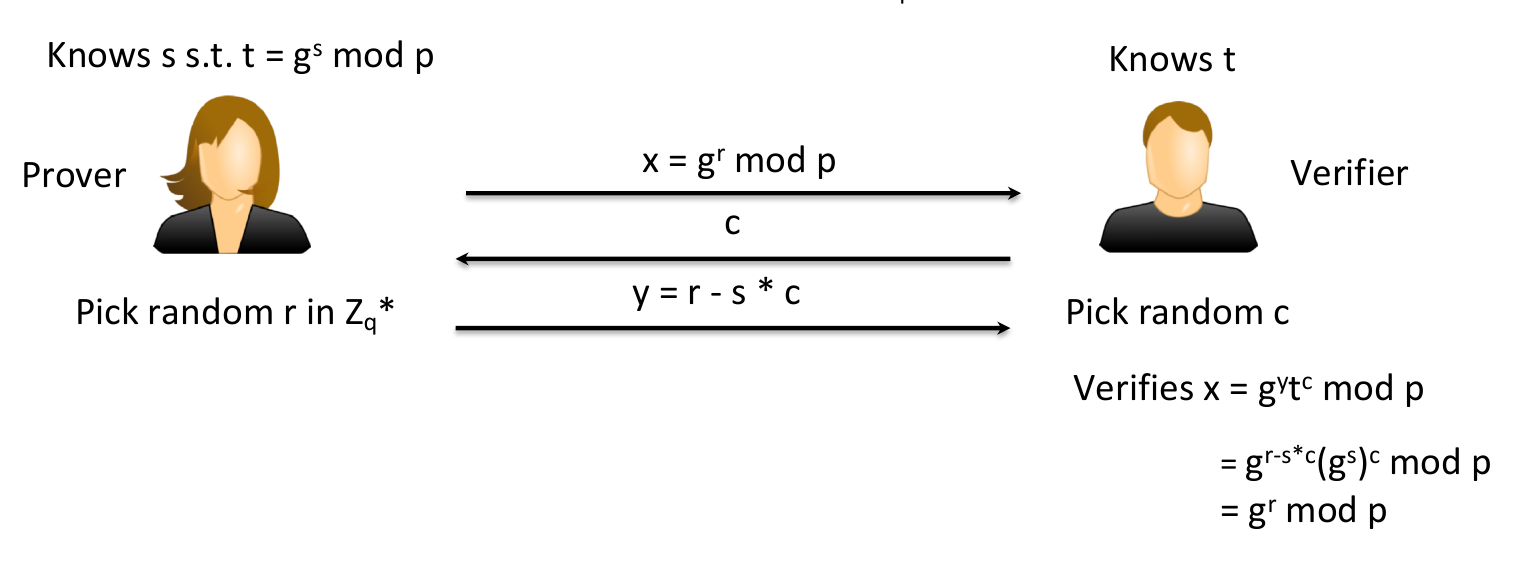
\includegraphics[width=12cm]{images/ch6-schnorr.png}
    \caption{Schnorr identification protocol}
    \label{fig:schnorr}
\end{figure}

\paragraph{Fiat-Shamir proof} proves the knowledge of the square root (of a public $t$) in the RSA group.

Public protocol parameters are: $n$ s.t $n=pq$ for large but unknown primes $p, q$.

\begin{figure}[h]
    \centering
    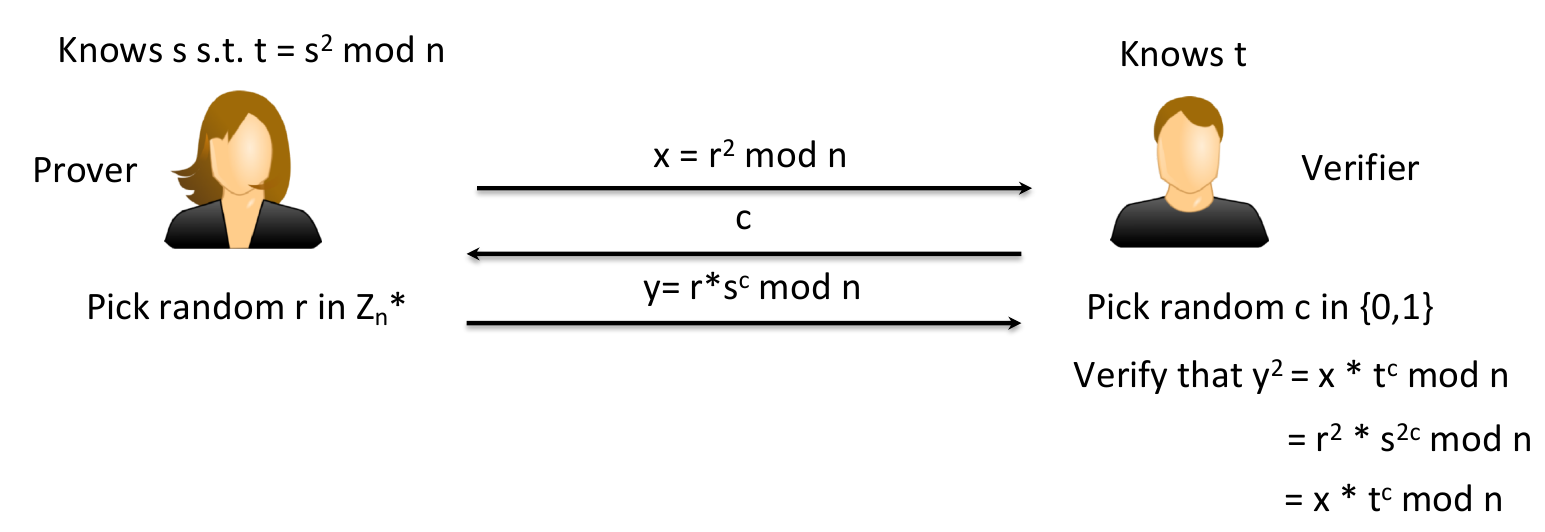
\includegraphics[width=12cm]{images/ch6-fiat-shamir.png}
    \caption{Fiat-Shamir proof}
    \label{fig:fiat-shamir}
\end{figure}


\pagebreak
\subsection{Commitment schemes}

\paragraph{Commitment scheme} Commit to a "hidden" value $x$ that cannot be changed later.

1\textsuperscript{st} stage $=$ commit: $P$ "locks" $x$ in a box and sends the box to V

2\textsuperscript{nd} stage $=$ reveal: $P$ gives the key to the box to $V$. $V$ opens the box and learns $x$.

\paragraph{Properties of commitment schemes}\mbox{}

\underline{Hiding:} After the commit phase, $V$ learns nothing about $x$

\underline{Binding:} After the commit phase, there is only one value (i.e. $x$) that $P$ can successfully reveal.

{ \scriptsize Exercise: Show that a commitment scheme can \textit{not} be both perfectly hiding and perfectly binding at the same time. }

\paragraph{Pedersen commitment scheme}
\begin{itemize}
    \item Setup (verifier)
    \begin{itemize}
        \item Pick primes $p$ and $q$ such that $q$ divides $p-1$
        \item Pick generators $g, h$ of the order-$q$ subgroup of $Z_p^*$ such that
            $$ a = \log_g(h) \Leftrightarrow h = g^a \mod p $$
        \item Public parameters: $p, q, g, h$, Secret: $a$
    \end{itemize}
    \item Commit (prover)
    \begin{itemize}
        \item Pick random $r \in Z_q$
        \item Output $c = g^x h^r \mod p$
    \end{itemize}
    \item Reveal (prover)
    \begin{itemize}
        \item Output $x, r$
     \end{itemize}
\end{itemize}

Note that $c$ is essentially a pseudo-random permutation of $x$.

Properties (intuition): Computationally binding because $g^x$ is hard to invert (discrete log). Perfectly hiding comes from the randomness of $h^r$.


% Slides contain the following sections that were not discussed by Prof Capkun: 
% - Pedersen Commitment – ZK Prove know how to open (without actually opening)
% - Bit proof protocol || explicitly stated to be not relevant
% - Elliptic curve crypto  || explicitly stated to be not relevant
% - Identity-based crypto  || explicitly stated to be not relevant
% Can be added - unlikely to be relevant for the FS20 exam
